% E02 · Especificación técnica de la solución (especificación v1.5, §15): arquitectura, datos, API y decisiones técnicas.
% Compilar: python EntregaFinal/documentos/compilar.py   (presupuesto: 12 a 16 páginas)
% Cifras: generado/cifras.tex (de api_frecuencias/docs/evidencias/); tabla de endpoints: generado/tabla_api.tex (de la
% aplicación FastAPI). Las rutas de evidencia son relativas a EntregaFinal/.
\documentclass[10pt,a4paper]{article}
\usepackage[a4paper,left=2cm,right=2cm,top=1.8cm,bottom=1.9cm,footskip=0.7cm]{geometry}
\newcommand{\piedepagina}{E02 · Especificación técnica · Sobusa – Extreme Technologies · Data Challenge 2026}
% Estilo común de E01 y E02: la letra (Inter, SIL OFL 1.1, en fuentes/) y los colores por rol del tablero
% (generado/colores.tex, que sale de dash_app/tokens.py). Ningún color se escribe aquí: solo roles.
\usepackage{fontspec}
% Sin las alternativas contextuales de Inter (calt): sus glifos de guion, dos puntos y paréntesis «de mayúscula» no
% tienen Unicode, y el texto copiado o extraído del PDF los perdía (2025-11-01 salía 20251101).
\defaultfontfeatures{Ligatures=TeX, RawFeature={-calt}}
\setmainfont{Inter-Regular.ttf}[Path=fuentes/, BoldFont=Inter-SemiBold.ttf, ItalicFont=Inter-Regular.ttf,
  ItalicFeatures={FakeSlant=0.16}, BoldItalicFont=Inter-SemiBold.ttf, BoldItalicFeatures={FakeSlant=0.16}]
\setsansfont{Inter-Regular.ttf}[Path=fuentes/, BoldFont=Inter-SemiBold.ttf, ItalicFont=Inter-Regular.ttf,
  ItalicFeatures={FakeSlant=0.16}]
\newfontfamily\interligera{Inter-Regular.ttf}[Path=fuentes/]
\newfontfamily\intermedia{Inter-Medium.ttf}[Path=fuentes/]
\usepackage[spanish,es-noshorthands,es-tabla,es-nodecimaldot]{babel}
\usepackage[table]{xcolor}
% Generado por documentos/datos_documentos.py desde dash_app/tokens.py (roles de DISENO.md §2).
\definecolor{rol-real}{RGB}{20,20,20}
\definecolor{rol-hoy}{RGB}{133,133,133}
\definecolor{rol-contexto}{RGB}{200,200,200}
\definecolor{rol-modelo}{RGB}{36,87,240}
\definecolor{rol-modelo-final}{RGB}{36,87,240}
\definecolor{rol-previsto-modelo}{RGB}{36,87,240}
\definecolor{rol-previsto-hoy}{RGB}{133,133,133}
\definecolor{rol-recorta}{RGB}{184,35,95}
\definecolor{rol-oraculo}{RGB}{20,20,20}
\definecolor{rol-modelo-tinte}{RGB}{220,229,253}
\definecolor{rol-hoy-tinte}{RGB}{227,227,227}
\definecolor{rol-recorta-tinte}{RGB}{246,219,230}
\definecolor{rol-referencia}{RGB}{102,102,102}
\definecolor{rol-cero}{RGB}{102,102,102}
\definecolor{rol-rejilla}{RGB}{235,235,235}
\definecolor{rol-eje}{RGB}{208,208,208}
\definecolor{rol-silencio}{RGB}{13,148,136}
\definecolor{rol-cra54}{RGB}{232,89,12}
\definecolor{rol-cl72}{RGB}{112,72,232}
\definecolor{rol-bien}{RGB}{24,117,58}
\definecolor{rol-atencion}{RGB}{178,111,11}
\definecolor{rol-atencion-texto}{RGB}{146,91,8}
\definecolor{rol-critico}{RGB}{186,43,46}
\definecolor{rol-acento}{RGB}{36,87,240}
\definecolor{rol-acento-fuerte}{RGB}{27,68,200}
\definecolor{rol-acento-suave}{RGB}{228,235,254}
\definecolor{rol-foco}{RGB}{36,87,240}
\definecolor{rol-tinta}{RGB}{20,20,20}
\definecolor{rol-tinta-2}{RGB}{85,85,85}
\definecolor{rol-tinta-3}{RGB}{102,102,102}
\definecolor{rol-tinta-tenue}{RGB}{138,138,138}
\definecolor{rol-tinta-inversa}{RGB}{255,255,255}
\definecolor{rol-blanco}{RGB}{255,255,255}
\definecolor{rol-superficie}{RGB}{250,250,250}
\definecolor{rol-superficie-2}{RGB}{233,233,233}
\definecolor{rol-fondo}{RGB}{239,239,239}
\definecolor{rol-linea}{RGB}{227,227,227}
\definecolor{rol-linea-fuerte}{RGB}{208,208,208}
\definecolor{rol-pantalla-inicio}{RGB}{20,20,20}
\definecolor{rol-pantalla-pronostico}{RGB}{20,20,20}
\definecolor{rol-pantalla-horario}{RGB}{20,20,20}
\definecolor{rol-pantalla-modelo}{RGB}{20,20,20}
\definecolor{rol-pantalla-resultado}{RGB}{20,20,20}
\definecolor{rol-pantalla-enlaces}{RGB}{20,20,20}

% Generado por documentos/datos_documentos.py: no editar a mano. Cada cifra con su evidencia.

\newcommand{\ModeloActivo}{hgb\_fv2\_20250831\_s42}% api_frecuencias/docs/evidencias/modelo/evaluacion_modelo.json
\newcommand{\PruebaDesde}{2025-11-01}% api_frecuencias/docs/evidencias/modelo/evaluacion_modelo.json
\newcommand{\PruebaHasta}{2025-12-31}% api_frecuencias/docs/evidencias/modelo/evaluacion_modelo.json
\newcommand{\Nprueba}{3.111}% api_frecuencias/docs/evidencias/modelo/evaluacion_modelo.json
\newcommand{\WAPEact}{14,77}% api_frecuencias/docs/evidencias/modelo/evaluacion_modelo.json
\newcommand{\MAEact}{96,27}% api_frecuencias/docs/evidencias/modelo/evaluacion_modelo.json
\newcommand{\WAPEactIC}{13,10--16,87}% api_frecuencias/docs/evidencias/modelo/evaluacion_modelo.json
\newcommand{\WAPEfvuno}{15,07}% api_frecuencias/docs/evidencias/modelo/evaluacion_modelo.json
\newcommand{\MAEfvuno}{98,20}% api_frecuencias/docs/evidencias/modelo/evaluacion_modelo.json
\newcommand{\WAPEfvunoIC}{13,22--17,43}% api_frecuencias/docs/evidencias/modelo/evaluacion_modelo.json
\newcommand{\WAPEbuno}{21,18}% api_frecuencias/docs/evidencias/modelo/evaluacion_modelo.json
\newcommand{\MAEbuno}{138,06}% api_frecuencias/docs/evidencias/modelo/evaluacion_modelo.json
\newcommand{\WAPEbunoIC}{16,61--26,79}% api_frecuencias/docs/evidencias/modelo/evaluacion_modelo.json
\newcommand{\WAPEbdos}{26,40}% api_frecuencias/docs/evidencias/modelo/evaluacion_modelo.json
\newcommand{\MAEbdos}{172,05}% api_frecuencias/docs/evidencias/modelo/evaluacion_modelo.json
\newcommand{\WAPEbdosIC}{22,77--30,57}% api_frecuencias/docs/evidencias/modelo/evaluacion_modelo.json
\newcommand{\SesgoAct}{2,75}% api_frecuencias/docs/evidencias/modelo/evaluacion_modelo.json
\newcommand{\DifActBunoIC}{−10,43 a −3,21}% api_frecuencias/docs/evidencias/modelo/evaluacion_modelo.json
\newcommand{\PmejoraActBuno}{1,00}% api_frecuencias/docs/evidencias/modelo/evaluacion_modelo.json
\newcommand{\MejoraRelBuno}{30}% api_frecuencias/docs/evidencias/modelo/evaluacion_modelo.json
\newcommand{\CobModelo}{79,49}% api_frecuencias/docs/evidencias/modelo/evaluacion_modelo.json
\newcommand{\CobConformal}{77,88}% api_frecuencias/docs/evidencias/modelo/evaluacion_modelo.json
\newcommand{\BajoPdiez}{13,28}% api_frecuencias/docs/evidencias/modelo/evaluacion_modelo.json
\newcommand{\SobrePnoventa}{8,84}% api_frecuencias/docs/evidencias/modelo/evaluacion_modelo.json
\newcommand{\WAPEPico}{14,38}% api_frecuencias/docs/evidencias/modelo/evaluacion_modelo.json
\newcommand{\WAPEValle}{14,97}% api_frecuencias/docs/evidencias/modelo/evaluacion_modelo.json
\newcommand{\WAPERutaSilencio}{15,33}% api_frecuencias/docs/evidencias/modelo/evaluacion_modelo.json
\newcommand{\WAPERutaSilencioBuno}{21,30}% api_frecuencias/docs/evidencias/modelo/evaluacion_modelo.json
\newcommand{\WAPERutaCra}{13,04}% api_frecuencias/docs/evidencias/modelo/evaluacion_modelo.json
\newcommand{\WAPERutaCraBuno}{19,79}% api_frecuencias/docs/evidencias/modelo/evaluacion_modelo.json
\newcommand{\WAPERutaCl}{19,23}% api_frecuencias/docs/evidencias/modelo/evaluacion_modelo.json
\newcommand{\WAPERutaClBuno}{25,27}% api_frecuencias/docs/evidencias/modelo/evaluacion_modelo.json
\newcommand{\RobDosmilveinticuatro}{16,26}% api_frecuencias/docs/evidencias/modelo/evaluacion_modelo.json
\newcommand{\RobDosmilveinticuatroIC}{14,97--17,91}% api_frecuencias/docs/evidencias/modelo/evaluacion_modelo.json
\newcommand{\RobDosmilveinticuatroBuno}{21,55}% api_frecuencias/docs/evidencias/modelo/evaluacion_modelo.json
\newcommand{\RobDosmilveinticinco}{14,48}% api_frecuencias/docs/evidencias/modelo/evaluacion_modelo.json
\newcommand{\RobDosmilveinticincoIC}{13,78--15,28}% api_frecuencias/docs/evidencias/modelo/evaluacion_modelo.json
\newcommand{\RobDosmilveinticincoBuno}{20,04}% api_frecuencias/docs/evidencias/modelo/evaluacion_modelo.json
\newcommand{\CobVdos}{77,82}% api_frecuencias/docs/evidencias/modelo/calibracion_condicional.json
\newcommand{\BajoPdiezVdos}{12,95}% api_frecuencias/docs/evidencias/modelo/calibracion_condicional.json
\newcommand{\SobrePnoventaVdos}{9,23}% api_frecuencias/docs/evidencias/modelo/calibracion_condicional.json
\newcommand{\AnchoVdos}{303,4}% api_frecuencias/docs/evidencias/modelo/calibracion_condicional.json
\newcommand{\CobVuno}{77,88}% api_frecuencias/docs/evidencias/modelo/calibracion_condicional.json
\newcommand{\BajoPdiezVuno}{13,28}% api_frecuencias/docs/evidencias/modelo/calibracion_condicional.json
\newcommand{\SobrePnoventaVuno}{8,84}% api_frecuencias/docs/evidencias/modelo/calibracion_condicional.json
\newcommand{\AnchoVuno}{312,9}% api_frecuencias/docs/evidencias/modelo/calibracion_condicional.json
\newcommand{\CalibPeorDesv}{4,15}% api_frecuencias/docs/evidencias/modelo/calibracion_condicional.json
\newcommand{\HorTreinta}{19,43}% api_frecuencias/docs/evidencias/modelo/horizontes.json
\newcommand{\HorTreintaBuno}{23,12}% api_frecuencias/docs/evidencias/modelo/horizontes.json
\newcommand{\HorSesenta}{14,71}% api_frecuencias/docs/evidencias/modelo/horizontes.json
\newcommand{\HorSesentaBuno}{18,96}% api_frecuencias/docs/evidencias/modelo/horizontes.json
\newcommand{\HorCientoveinte}{10,87}% api_frecuencias/docs/evidencias/modelo/horizontes.json
\newcommand{\HorCientoveinteBuno}{15,44}% api_frecuencias/docs/evidencias/modelo/horizontes.json
\newcommand{\HorEvaluado}{2025-03-01 a 2025-12-31}% api_frecuencias/docs/evidencias/modelo/horizontes.json
\newcommand{\AlertasAhora}{0,53}% api_frecuencias/docs/evidencias/alertas/backtest_alertas.json
\newcommand{\AlertasAntes}{6,08}% api_frecuencias/docs/evidencias/alertas/backtest_alertas.json
\newcommand{\AlertasObsTodas}{1,24}% api_frecuencias/docs/evidencias/alertas/backtest_alertas.json
\newcommand{\DiasRuta}{324}% api_frecuencias/docs/evidencias/alertas/backtest_alertas.json
\newcommand{\AlertasDesde}{2025-09-15}% api_frecuencias/docs/evidencias/alertas/backtest_alertas.json
\newcommand{\AlertasHasta}{2025-12-31}% api_frecuencias/docs/evidencias/alertas/backtest_alertas.json
\newcommand{\LiftCinco}{4,69}% api_frecuencias/docs/evidencias/alertas/backtest_alertas.json
\newcommand{\LiftAntesCinco}{1,77}% api_frecuencias/docs/evidencias/alertas/backtest_alertas.json
\newcommand{\PrecCinco}{0,36}% api_frecuencias/docs/evidencias/alertas/backtest_alertas.json
\newcommand{\LiftSeis}{8,30}% api_frecuencias/docs/evidencias/alertas/backtest_alertas.json
\newcommand{\LiftAntesSeis}{1,31}% api_frecuencias/docs/evidencias/alertas/backtest_alertas.json
\newcommand{\PrecSeis}{0,39}% api_frecuencias/docs/evidencias/alertas/backtest_alertas.json
\newcommand{\LiftSiete}{1,34}% api_frecuencias/docs/evidencias/alertas/backtest_alertas.json
\newcommand{\LiftAntesSiete}{0,78}% api_frecuencias/docs/evidencias/alertas/backtest_alertas.json
\newcommand{\PrecSiete}{0,27}% api_frecuencias/docs/evidencias/alertas/backtest_alertas.json
\newcommand{\LiftOcho}{3,78}% api_frecuencias/docs/evidencias/alertas/backtest_alertas.json
\newcommand{\LiftAntesOcho}{2,87}% api_frecuencias/docs/evidencias/alertas/backtest_alertas.json
\newcommand{\PrecOcho}{0,70}% api_frecuencias/docs/evidencias/alertas/backtest_alertas.json
\newcommand{\UOcupCritica}{0,90}% api_frecuencias/docs/evidencias/alertas/backtest_alertas.json
\newcommand{\UBajaUtil}{0,30}% api_frecuencias/docs/evidencias/alertas/backtest_alertas.json
\newcommand{\UCaida}{0,30}% api_frecuencias/docs/evidencias/alertas/backtest_alertas.json
\newcommand{\UPersistencia}{2}% api_frecuencias/docs/evidencias/alertas/backtest_alertas.json
\newcommand{\UErrorPron}{0,15}% api_frecuencias/docs/evidencias/alertas/backtest_alertas.json
\newcommand{\UZ}{3,5}% api_frecuencias/docs/evidencias/alertas/backtest_alertas.json
\newcommand{\UTolDespacho}{5}% api_frecuencias/docs/evidencias/alertas/backtest_alertas.json
\newcommand{\UTolSalidas}{0,50}% api_frecuencias/docs/evidencias/alertas/backtest_alertas.json
\newcommand{\UAtraso}{2}% api_frecuencias/docs/evidencias/alertas/backtest_alertas.json
\newcommand{\UWapeMax}{0,20}% api_frecuencias/docs/evidencias/alertas/backtest_alertas.json
\newcommand{\USemanasRef}{8}% api_frecuencias/docs/evidencias/alertas/backtest_alertas.json
\newcommand{\UTolSalidasPct}{50}% api_frecuencias/docs/evidencias/alertas/backtest_alertas.json
\newcommand{\UUnoMenosCaida}{0,70}% api_frecuencias/docs/evidencias/alertas/backtest_alertas.json
\newcommand{\AlertasAhoraDosmil}{0,45}% api_frecuencias/docs/evidencias/alertas/backtest_alertas_corte_2024-12-31.json
\newcommand{\AlertasAntesDosmil}{5,70}% api_frecuencias/docs/evidencias/alertas/backtest_alertas_corte_2024-12-31.json
\newcommand{\AlertasPronUno}{0,44}% api_frecuencias/docs/evidencias/alertas/backtest_alertas_pronostico.json
\newcommand{\AlertasPronDos}{0,32}% api_frecuencias/docs/evidencias/alertas/backtest_alertas_pronostico.json
\newcommand{\AlertasPronTres}{0,38}% api_frecuencias/docs/evidencias/alertas/backtest_alertas_pronostico.json
\newcommand{\AlertasPronCuatro}{0,03}% api_frecuencias/docs/evidencias/alertas/backtest_alertas_pronostico.json
\newcommand{\AlertasPronostico}{1,16}% api_frecuencias/docs/evidencias/alertas/backtest_alertas_pronostico.json
\newcommand{\AlertasTotal}{2,40}% api_frecuencias/docs/evidencias/alertas/backtest_alertas_pronostico.json
\newcommand{\ViablesBacktest}{46,0}% api_frecuencias/docs/evidencias/alertas/backtest_alertas_pronostico.json
\newcommand{\RevisionDoble}{dos revisores automatizados con un protocolo escrito, conciliación y kappa de Cohen de 0,80}% api_frecuencias/docs/evidencias/alertas/revision_doble/conciliacion.json
\newcommand{\Kpnoventaycinco}{451}% api_frecuencias/docs/evidencias/pruebas/k6_consultas.json
\newcommand{\Kpnoventaynueve}{572}% api_frecuencias/docs/evidencias/pruebas/k6_consultas.json
\newcommand{\Kpeticiones}{3.553}% api_frecuencias/docs/evidencias/pruebas/k6_consultas.json
\newcommand{\Ktasa}{58,8}% api_frecuencias/docs/evidencias/pruebas/k6_consultas.json
\newcommand{\Kerrores}{0,00}% api_frecuencias/docs/evidencias/pruebas/k6_consultas.json
\newcommand{\Kvus}{50}% api_frecuencias/docs/evidencias/pruebas/k6_consultas.json
\newcommand{\Kingesta}{722}% api_frecuencias/docs/evidencias/pruebas/k6_ingesta.json
\newcommand{\IngestaFilas}{111.792}% api_frecuencias/docs/evidencias/rendimiento.txt
\newcommand{\IngestaSegundos}{4,07}% api_frecuencias/docs/evidencias/rendimiento.txt
\newcommand{\IngestaTasa}{27.469}% api_frecuencias/docs/evidencias/rendimiento.txt
\newcommand{\IngestaMemoria}{53}% api_frecuencias/docs/evidencias/rendimiento.txt
\newcommand{\Ntotal}{1.060}% api_frecuencias/docs/evidencias/pruebas/suite_final.xml
\newcommand{\Npasan}{1.055}% api_frecuencias/docs/evidencias/pruebas/suite_final.xml
\newcommand{\Nfallan}{0}% api_frecuencias/docs/evidencias/pruebas/suite_final.xml
\newcommand{\Nomitidas}{5}% api_frecuencias/docs/evidencias/pruebas/suite_final.xml
\newcommand{\NUnit}{567}% api_frecuencias/docs/evidencias/pruebas/suite_final.xml
\newcommand{\NInteg}{106}% api_frecuencias/docs/evidencias/pruebas/suite_final.xml
\newcommand{\NReplica}{185}% api_frecuencias/docs/evidencias/pruebas/suite_final.xml
\newcommand{\NContrato}{178}% api_frecuencias/docs/evidencias/pruebas/suite_final.xml
\newcommand{\NDatos}{24}% api_frecuencias/docs/evidencias/pruebas/suite_final.xml
\newcommand{\NTcont}{8}% api_frecuencias/docs/evidencias/pruebas/ci/pytest.xml
\newcommand{\NTcontNota}{ (en su trabajo del CI)}% api_frecuencias/docs/evidencias/pruebas/ci/pytest.xml
\newcommand{\FechaPruebas}{2026-11-09 12:37}% api_frecuencias/docs/evidencias/pruebas/suite_final.xml
\newcommand{\CorridaPruebas}{corrida final de la suite completa (2026-11-09 12:37)}% api_frecuencias/docs/evidencias/pruebas/suite_final.xml
\newcommand{\Cobertura}{94,3}% api_frecuencias/docs/evidencias/pruebas/coverage_final.xml
\newcommand{\NIntentosLector}{32}% api_frecuencias/docs/evidencias/pruebas/suite_final.xml
\newcommand{\NIntentosEscritor}{84}% api_frecuencias/docs/evidencias/pruebas/suite_final.xml
\newcommand{\NIntentosTotal}{116}% api_frecuencias/docs/evidencias/pruebas/suite_final.xml
\newcommand{\FuenteIntentos}{\path{api_frecuencias/docs/evidencias/pruebas/suite_final.xml}}% api_frecuencias/docs/evidencias/pruebas/suite_final.xml
\newcommand{\EstadoCI}{en verde en GitHub Actions (run 42627652053, 2026-11-09)}% api_frecuencias/docs/evidencias/pruebas/ci_github.txt
\newcommand{\EstadoCICorto}{en verde en GitHub Actions (run 42627652053, 2026-11-09)}% api_frecuencias/docs/evidencias/pruebas/ci_github.txt
\newcommand{\GateCandidato}{hgb\_fv1\_20250831\_s42}% api_frecuencias/docs/evidencias/monitoreo/compuerta_ejemplo.json
\newcommand{\GateWAPECand}{12,97}% api_frecuencias/docs/evidencias/monitoreo/compuerta_ejemplo.json
\newcommand{\GateWAPEAct}{13,02}% api_frecuencias/docs/evidencias/monitoreo/compuerta_ejemplo.json
\newcommand{\GateDecision}{aprobado}% api_frecuencias/docs/evidencias/monitoreo/compuerta_ejemplo.json
\newcommand{\GateVentana}{2025-09-01 a 2025-09-14}% api_frecuencias/docs/evidencias/monitoreo/compuerta_ejemplo.json
\newcommand{\NVariables}{23}% api_frecuencias/docs/evidencias/monitoreo/onnx_paridad.json
\newcommand{\FeatureVersion}{fv2-2026-11-09}% api_frecuencias/docs/evidencias/monitoreo/onnx_paridad.json
\newcommand{\OnnxDifMax}{0,0028}% api_frecuencias/docs/evidencias/monitoreo/onnx_paridad.json
\newcommand{\OnnxMsFila}{0,10}% api_frecuencias/docs/evidencias/monitoreo/onnx_paridad.json
\newcommand{\SklearnMsFila}{12,6}% api_frecuencias/docs/evidencias/monitoreo/onnx_paridad.json
\newcommand{\FranjasTotal}{13}% api_frecuencias/docs/evidencias/optimizacion/sensibilidad.md
\newcommand{\FranjasViables}{11}% api_frecuencias/docs/evidencias/optimizacion/sensibilidad.md
\newcommand{\FranjasMilpIgual}{13}% api_frecuencias/docs/evidencias/optimizacion/sensibilidad.md
\newcommand{\FranjasNoViables}{CRA 54 (laboral, 7~h) y CRA 54 (sábado, 7~h)}% api_frecuencias/docs/evidencias/optimizacion/sensibilidad.md
\newcommand{\PlanRuta}{CRA 54}% api_frecuencias/docs/evidencias/optimizacion/ejemplo_plan_d5.json
\newcommand{\PlanFecha}{2025-11-19}% api_frecuencias/docs/evidencias/optimizacion/ejemplo_plan_d5.json
\newcommand{\PlanSalidas}{247}% api_frecuencias/docs/evidencias/optimizacion/ejemplo_plan_d5.json
\newcommand{\PlanProgramadas}{290,2}% api_frecuencias/docs/evidencias/optimizacion/ejemplo_plan_d5.json
\newcommand{\PlanHoraPico}{5}% api_frecuencias/docs/evidencias/optimizacion/ejemplo_plan_d5.json
\newcommand{\PlanHeadwayPico}{2,0}% api_frecuencias/docs/evidencias/optimizacion/ejemplo_plan_d5.json
\newcommand{\PlanSalidasPico}{30}% api_frecuencias/docs/evidencias/optimizacion/ejemplo_plan_d5.json
\newcommand{\PlanHeadwayMax}{8,5}% api_frecuencias/docs/evidencias/optimizacion/ejemplo_plan_d5.json
\newcommand{\SonarResumen}{SonarQube: puerta de calidad aprobada (vulnerabilidades: 0; errores: 0; bloqueantes: 0; críticos: 0; duplicación: 0,0~\%; cobertura: 94,3~\%)}% api_frecuencias/docs/evidencias/sonarqube/measures.json
\newcommand{\SonarCorto}{SonarQube: puerta de calidad aprobada (vulnerabilidades: 0; errores: 0; bloqueantes: 0; críticos: 0)}% api_frecuencias/docs/evidencias/sonarqube/measures.json
\newcommand{\SonarPuerta}{puerta de calidad aprobada}% api_frecuencias/docs/evidencias/sonarqube/measures.json
\newcommand{\SonarPruebas}{1.055}% api_frecuencias/docs/evidencias/sonarqube/measures.json
\newcommand{\DemoFilasInicial}{49.623}% api_frecuencias/docs/evidencias/despliegue/demo_ciclo_api.txt
\newcommand{\DemoFilasNuevas}{51}% api_frecuencias/docs/evidencias/despliegue/demo_ciclo_api.txt
\newcommand{\DemoFilasRepeticion}{0}% api_frecuencias/docs/evidencias/despliegue/demo_ciclo_api.txt
\newcommand{\DemoMarcaAntes}{2025-08-30}% api_frecuencias/docs/evidencias/despliegue/demo_ciclo_api.txt
\newcommand{\DemoMarcaDespues}{2025-08-31}% api_frecuencias/docs/evidencias/despliegue/demo_ciclo_api.txt
\newcommand{\DemoWapeNuevo}{26,5}% api_frecuencias/docs/evidencias/despliegue/demo_ciclo_api.txt
\newcommand{\DemoCandidato}{hgb\_fv2\_20250930\_s42}% api_frecuencias/docs/evidencias/despliegue/demo_ciclo_api.txt
\newcommand{\DemoEntrenoSeg}{37}% api_frecuencias/docs/evidencias/despliegue/demo_ciclo_api.txt
\newcommand{\DemoWapeCand}{14,11}% api_frecuencias/docs/evidencias/despliegue/demo_ciclo_api.txt
\newcommand{\DemoWapeAct}{13,98}% api_frecuencias/docs/evidencias/despliegue/demo_ciclo_api.txt
\newcommand{\DemoVentana}{2025-12-01 a 2025-12-14}% api_frecuencias/docs/evidencias/despliegue/demo_ciclo_api.txt
\newcommand{\DemoDecision}{rechazado}% api_frecuencias/docs/evidencias/despliegue/demo_ciclo_api.txt
\newcommand{\DemoTotalSeg}{190}% api_frecuencias/docs/evidencias/despliegue/demo_ciclo_api.txt
\newcommand{\PlanSemanasConexion}{1--4}% PLAN_EVOLUCION.md
\newcommand{\PlanSemanasSombra}{5--8}% PLAN_EVOLUCION.md
\newcommand{\PlanSemanasPiloto}{9--16}% PLAN_EVOLUCION.md
\newcommand{\PlanSemanasSombraTexto}{las semanas 5 a 8}% PLAN_EVOLUCION.md
\newcommand{\PlanSemanasPilotoTexto}{las semanas 9 a 16}% PLAN_EVOLUCION.md
\newcommand{\PlanHallazgosUrgentes}{H3, H6, H7, H9, H13 y H14}% PLAN_EVOLUCION.md
\newcommand{\PlanCriterioSombra}{WAPE \ensuremath{\le} 15 \% a 60 min, \ensuremath{\le} 20 \% a 30 min y \ensuremath{\le} 15 \% a 120 min, y por debajo de B1, en las cuatro semanas; menos del 30 \% de alertas descartadas}% PLAN_EVOLUCION.md
\newcommand{\PlanCostoComputo}{50--80}% PLAN_EVOLUCION.md
\newcommand{\PlanCostoBase}{(A) 0 · (B) 70--150}% PLAN_EVOLUCION.md
\newcommand{\PlanCostoReplica}{(A) 0 · (B) 70--150}% PLAN_EVOLUCION.md
\newcommand{\PlanCostoTotalA}{60--105}% PLAN_EVOLUCION.md
\newcommand{\PlanCostoTotalB}{200--405}% PLAN_EVOLUCION.md
\newcommand{\HallazgosRango}{H1--H16}% api_frecuencias/docs/hallazgos_extreme.md
\newcommand{\NHallazgos}{16}% api_frecuencias/docs/hallazgos_extreme.md
\newcommand{\NHallazgosTexto}{dieciséis}% api_frecuencias/docs/hallazgos_extreme.md
\newcommand{\FuentePruebas}{\path{api_frecuencias/docs/evidencias/pruebas/suite_final.xml}}
\newcommand{\FuenteCobertura}{\path{api_frecuencias/docs/evidencias/pruebas/coverage_final.xml}}

% Generado por documentos/tabla_api.py desde la aplicación FastAPI (app.main). No editar a mano.
\newcommand{\NOperaciones}{62}
\newcommand{\NOperacionesVuno}{60}
\newcommand{\VersionAPI}{1.0.0}
\newcommand{\OrigenTablaAPI}{la aplicación FastAPI (app.main)}

% Generado por documentos/datos_documentos.py desde api_frecuencias/docs/evidencias/respuesta/respuesta_2025-11-19.json. No editar a mano.
\newcommand{\RespuestaDisponible}{1}
\newcommand{\RespuestaFecha}{2025-11-19}
\newcommand{\RespuestaTipoDia}{Laboral}
\newcommand{\RespuestaModelo}{hgb\_fv2\_20250831\_s42}
\newcommand{\RespuestaFuentePronostico}{modelo\ activo}
\newcommand{\RespuestaFuente}{\path{respuesta_2025-11-19.json}}
\newcommand{\RespuestaNoViables}{1}
\newcommand{\RespuestaHoras}{51}
\newcommand{\RespuestaFilas}{%
SILENCIO & 135 / 158,5 & 8,18 / 8,00 / 9,97\newline\textcolor{rol-tinta-3}{hoy 6,86 / 6,77 / 7,26} & ninguna & 11.469 (8.458--14.160) & 44 / 45 & 36,5 / 31,3 \\
CRA 54 & 247 / 290,2 & 3,00 / 4,00 / 7,46\newline\textcolor{rol-tinta-3}{hoy 2,87 / 3,50 / 3,93} & 5~h & 22.800 (19.054--26.560) & 79 / 79 & 72,5 / 52,9 \\
CL 72 & 110 / 96,5 & 10,00 / 9,41 / 9,97\newline\textcolor{rol-tinta-3}{hoy 10,13 / 11,61 / 12,03} & ninguna & 7.525 (5.320--9.628) & 30 / 45 & 23,9 / 23,9 \\
}
\newcommand{\RespEjRuta}{CRA 54}
\newcommand{\RespEjSalidas}{247}
\newcommand{\RespEjProgramadas}{290,2}
\newcommand{\RespEjPicoManana}{3,00}
\newcommand{\RespEjValle}{4,00}
\newcommand{\RespEjPicoTarde}{7,46}
\newcommand{\RespEjNoViables}{a las 5~h la hora sale \emph{no viable}, con su motivo y la mejor aproximación ejecutable}
\newcommand{\RespuestaEjemplo}{CRA 54: ALT-006 crítica, «En 12:00-20:00 (8 h): salieron 17 de 136 despachos esperados (60 / intervalo programado).» Recomendación: Verificar la disponibilidad del vehículo y la operación del despacho.}
\newcommand{\RespuestaEjemploFuente}{\path{respuesta_2025-11-19.json}}

\usepackage{graphicx}
\graphicspath{{figuras/}{../informe/figuras/}}
\usepackage{booktabs,array,tabularx,longtable,multirow}
\usepackage{enumitem}
\usepackage{amsmath}
\usepackage{xurl}
\usepackage[hidelinks]{hyperref}
\usepackage{caption}
\usepackage{tikz}
\usetikzlibrary{positioning,arrows.meta,fit,backgrounds,calc}
\usepackage[most]{tcolorbox}
\usepackage{titlesec}
\usepackage{fancyhdr}
\usepackage{lastpage}

\color{rol-tinta}
\hypersetup{colorlinks=true, linkcolor=rol-acento-fuerte, urlcolor=rol-acento-fuerte, citecolor=rol-acento-fuerte,
  pdfauthor={Abrahan Basto Martínez, Rubén Esguerra Fernández, Paula Gómez}, pdflang={es-CO},
  pdfsubject={Data Challenge 2026 - Extreme Technologies y Universidad del Norte}}
\captionsetup{font={small,color=rol-tinta-2}, labelfont={color=rol-tinta}, justification=raggedright,
  singlelinecheck=false}
\setlist{nosep, leftmargin=1.2em}
\setlength{\parskip}{3pt plus 1pt}
\setlength{\parindent}{0pt}
\renewcommand{\arraystretch}{1.12}
\arrayrulecolor{rol-linea-fuerte}
\widowpenalty=10000 \clubpenalty=10000
\setlength{\emergencystretch}{3em}   % los identificadores largos (\texttt) bajan de línea en vez de salirse
% Texto alineado a la izquierda, como el tablero: los identificadores largos no fuerzan espacios enormes ni se salen.
\usepackage{ragged2e}
\AtBeginDocument{\RaggedRight\hyphenpenalty=5000\exhyphenpenalty=5000}   % casi sin guiones, como el tablero

% Títulos en peso normal (zentra: título grande en 400) y el número en gris.
\titleformat{\section}{\interligera\Large\color{rol-tinta}}{\textcolor{rol-tinta-3}{\thesection}}{0.6em}{}
\titleformat{\subsection}{\intermedia\normalsize\color{rol-tinta}}{\textcolor{rol-tinta-3}{\thesubsection}}{0.5em}{}
\titleformat{\paragraph}[runin]{\intermedia\color{rol-tinta}}{}{0pt}{}[.]
\titlespacing*{\section}{0pt}{10pt plus 2pt}{4pt}
\titlespacing*{\subsection}{0pt}{7pt plus 2pt}{2pt}
\titlespacing*{\paragraph}{0pt}{4pt}{0.6em}

% Fuente de una cifra, tabla o figura: la ruta de la evidencia, relativa a EntregaFinal/.
\newcommand{\fuente}[1]{{\footnotesize\color{rol-tinta-3}Fuente: \path{#1}}}
\newcommand{\evid}[1]{{\footnotesize\color{rol-tinta-3}\path{#1}}}
\newcommand{\evidt}[2]{{\footnotesize\color{rol-tinta-3}\path{#1}, #2}}
\newcommand{\dato}[1]{\textcolor{rol-acento-fuerte}{#1}}
\newcommand{\tenue}[1]{\textcolor{rol-tinta-2}{#1}}

% Tarjeta zentra: superficie casi blanca, borde fino y esquinas redondeadas.
\newtcolorbox{tarjeta}[1][]{enhanced, breakable, colback=rol-superficie, colframe=rol-linea, boxrule=0.6pt, arc=8pt,
  left=8pt, right=8pt, top=6pt, bottom=6pt, #1}
\newtcolorbox{respuesta}[1][]{enhanced, colback=rol-acento-suave, colframe=rol-acento-suave, boxrule=0pt, arc=8pt,
  left=9pt, right=9pt, top=6pt, bottom=6pt, #1}

\pagestyle{fancy}
\fancyhf{}
\renewcommand{\headrulewidth}{0pt}
\fancyfoot[L]{\footnotesize\color{rol-tinta-3}\piedepagina}
\fancyfoot[R]{\footnotesize\color{rol-tinta-3}\thepage\ de \pageref*{LastPage}}

\setcounter{tocdepth}{1}

\hypersetup{pdftitle={E02 Especificación técnica - Sistema de pronóstico y frecuencias de despacho}}
\begin{document}
\thispagestyle{fancy}
{\footnotesize\color{rol-tinta-3}E02 · ESPECIFICACIÓN TÉCNICA DE LA SOLUCIÓN \hfill versión de la API \VersionAPI{} · 9 de
noviembre de 2026}\par\vspace{4pt}
{\interligera\fontsize{22}{26}\selectfont Sistema de pronóstico y frecuencias de despacho\par}
\vspace{2pt}
{\large\tenue{Arquitectura, datos, modelo, optimización, alertas, base de datos, integración, API, requisitos no
funcionales, pruebas, seguridad y decisiones técnicas}\par}
\vspace{4pt}
{\small Abrahan Basto Martínez · Rubén Esguerra Fernández · Paula Gómez — Universidad del Norte, para Extreme
Technologies (especificación v1.5).\par}
\vspace{6pt}

\begin{tarjeta}
\small\textbf{Cómo leer este documento.} Cada sección corresponde a un apartado de la especificación v1.5 (entre
paréntesis). Cada cifra cita el archivo de evidencia que la produjo, con la ruta relativa a la carpeta
\path{EntregaFinal/}; el código está en \path{api_frecuencias/} (paquete \path{app/}, migraciones en
\path{alembic/versions/}, pruebas en \path{tests/}). La tabla de endpoints de la sección~\ref{sec:api} se genera desde
la propia aplicación FastAPI, así que no puede desviarse del código. Los manuales técnico, de usuario y de despliegue
están en \path{api_frecuencias/docs/}.
\end{tarjeta}

{\small\tableofcontents}

% ------------------------------------------------------------------------------------------------------------------
\section{Alcance y supuestos (§1--§3, §19)}
El sistema responde la pregunta de §20 para las rutas SILENCIO, CRA~54 y CL~72 con los datos de 2023 a 2025: cada día
lee lo nuevo de las tablas de Extreme, valida su calidad, pronostica los pasajeros por ruta y hora (horizontes de 30, 60
y 120 minutos) con su incertidumbre, recomienda el intervalo de despacho, los buses por hora y los vehículos, evalúa
diez reglas de alerta y deja todo en el esquema \texttt{ai\_frecuencias} con su trazabilidad. Lo exponen
\NOperaciones{} operaciones REST y un tablero. Cumple los seis módulos de §3.1 y respeta §3.2: no controla despachos ni
vehículos, no toca triggers ni tablas operativas y no se declara listo para producción sin la prueba de Extreme.

\textbf{Supuestos hasta que Extreme entregue lo de §19.} Capacidad, tiempo de ciclo, flota por franja e intervalo
programado se derivan de los datos (\path{datos/parametros_operativos_hora.parquet}); las tipologías de capacidad
salen del reporte de flota sin placas (\path{app/servicios/tipologias_flota.json}); los umbrales de §5.1 y los pesos de
la función objetivo de §10.2 empiezan en los valores sugeridos y viven versionados en
\texttt{ai\_frecuencias.threshold\_config}, donde el área operativa los cambia sin recompilar. La espera máxima de §5.1
se interpreta como espera media del pasajero (headway / 2 con llegadas aleatorias), así que el headway máximo efectivo
es el menor entre \texttt{headway\_maximo\_min} y dos veces \texttt{espera\_max\_min}, en la recomendación de franja y
en el plan del día (supuesto S12 de \path{documentos/mapeo_especificacion.md}, con su pregunta a Extreme). Los
\NHallazgosTexto{} hallazgos sobre los datos y scripts de Extreme (\HallazgosRango,
\path{api_frecuencias/docs/hallazgos_extreme.md}) están documentados con la pregunta exacta que hay que hacerles.

% ------------------------------------------------------------------------------------------------------------------
\section{Arquitectura (§7)}
\label{sec:arquitectura}
La solución separa ingesta, dominio operacional, analítica, inferencia, optimización, alertas y exposición (§7.1). La
figura~\ref{fig:arquitectura} muestra el recorrido de un dato: las tablas de Extreme siguen alimentadas por sus
triggers; un adaptador de solo lectura toma lo nuevo; un trabajo en cola corre el ciclo; los resultados se escriben con
otro usuario y solo en \texttt{ai\_frecuencias}; la API los sirve y el tablero los muestra. Al cerrar cada ejecución
diaria, el ciclo calcula con el modelo activo el plan del día siguiente por ruta y hora y la foto de la respuesta del
reto, y los guarda (\texttt{recommendation} con origen \texttt{plan\_dia} y \texttt{respuesta\_reto}). Así
\texttt{GET /api/v1/recommendations/plan} y \texttt{GET /api/v1/respuesta} solo leen lo calculado: si una fecha no
está, responden 404 \texttt{sin\_calcular} y \texttt{POST /api/v1/respuesta/calcular} (analista) la encola y responde
202 con el \texttt{execution\_id} (§7.1, procesos largos asíncronos). Las tablas de resultados llevan las dimensiones
de §8.3 (\texttt{idruta}, \texttt{idempresa}, \texttt{idproceso}, \texttt{id\_dia\_semana} e
\texttt{id\_estacionalidad}) y la API filtra por \texttt{idruta}.

\begin{figure}[ht]
\centering
\begin{tikzpicture}[
  font=\footnotesize, node distance=4mm and 7mm,
  caja/.style={draw=rol-linea-fuerte, fill=rol-superficie, rounded corners=5pt, align=left, inner sep=4pt,
    text width=#1},
  caja/.default=3.6cm,
  nuestra/.style={caja=#1, draw=rol-modelo, fill=rol-acento-suave},
  nuestra/.default=3.6cm,
  flecha/.style={-{Stealth[length=2.2mm]}, draw=rol-tinta-2, line width=0.7pt},
  rot/.style={font=\scriptsize, text=rol-tinta-2, fill=white, inner sep=1pt}]
\node[caja=3.5cm] (ext) {\textbf{PostgreSQL 14 de Extreme}\\
  \texttt{timbradas\_segmentos}, \texttt{timbradas\_anio}, \texttt{timbradas\_consolidado}, \texttt{rutas},
  \texttt{progvehiculos}, \texttt{novedades\_viales*}, segmentos\\[2pt]
  \tenue{triggers, funciones y scripts sin cambios (RF-002); réplica de lectura recomendada (§11.3)}};
\node[nuestra=3.9cm, right=19mm of ext.north east, anchor=north west] (fuente) {\textbf{Adaptador de solo lectura}
  (\path{app/servicios/fuentes.py})\\ lista blanca de SELECT, \texttt{READ ONLY}, \texttt{statement\_timeout},
  zona America/Bogota; marca de agua + solape de 15 min + huella md5; circuit breaker};
\node[nuestra=3.9cm, below=of fuente] (cola) {\textbf{Cola de trabajos en PostgreSQL} (\path{cola.py})\\
  \texttt{FOR UPDATE SKIP LOCKED}, reintentos, progreso; planificador diario y semanal (\path{planificador.py})};
\node[nuestra=3.9cm, below=of cola] (ciclo) {\textbf{Ciclo de frecuencia} (\path{ejecucion.py})\\
  1 calidad (§6.3) · 2 variables fv2 · 3 inferencia (modelo activo, banda calibrada) · 4 optimización MILP ·
  5 alertas ALT-001..010 con escalamiento · 6 monitoreo y política · 7 plan del día siguiente y foto de la respuesta};
\node[nuestra=3.5cm, anchor=north west] (ai) at (ext.west |- ciclo.north) {\textbf{PostgreSQL 14 + PostGIS}\\
  esquema \texttt{ai\_frecuencias} (Alembic): predicciones, recomendaciones y plan del día, alertas, bitácora,
  ejecuciones, modelos, umbrales, monitoreo, foto de variables, respuesta del reto; dimensiones de §8.3};
\node[nuestra=3.5cm, anchor=south west] (api) at ($(fuente.east |- ciclo.south)+(10mm,0)$) {\textbf{API FastAPI}
  \texttt{/api/v1}\\ \NOperacionesVuno{} operaciones con OpenAPI 3, claves por rol, errores uniformes, paginación,
  exportación CSV/XLSX; procesos largos en cola (202); sin estado: N réplicas};
\node[caja=3.5cm, above=of api] (dash) {\textbf{Tablero Dash} y clientes\\ alertas, recomendaciones, operación
  (modelos, umbrales, monitoreo), despacho en vivo};
\node[caja=3.5cm, above=of dash] (obs) {\textbf{Observabilidad}\\ logs JSON con \texttt{correlation\_id}
  (structlog), \texttt{/metrics} (Prometheus), trazas OpenTelemetry (Jaeger), \texttt{/health}};
\draw[flecha] ($(ext.east)+(0,0.3)$) -- node[rot, above] {\texttt{lector\_ia}} ($(fuente.west |- ext.east)+(0,0.3)$);
\draw[flecha] (fuente) -- (cola);
\draw[flecha] (cola) -- (ciclo);
\draw[flecha] ($(ciclo.west)+(0,0.2)$) -- node[rot, above] {\texttt{escritor\_ia}} ($(ai.east |- ciclo.west)+(0,0.2)$);
\draw[flecha] (ai.south) -- ++(0,-0.35) -| node[rot, pos=0.25, below] {la API lee sus resultados} (api.south);
\draw[flecha] (api) -- (dash);
\end{tikzpicture}
\caption{Arquitectura. Azul: lo que construimos; gris: lo que existe en Extreme o lo consume. El usuario de lectura
nunca escribe y el de escritura solo toca \texttt{ai\_frecuencias} (comprobado en la réplica,
sección~\ref{sec:integracion}).}
\label{fig:arquitectura}
\end{figure}

\begin{table}[ht]
\centering\small
\caption{Componentes lógicos de §7.2 y dónde están.}
\label{tab:componentes}
\begin{tabularx}{\linewidth}{@{}l>{\raggedright\arraybackslash}p{4.4cm}X@{}}
\toprule
Componente (§7.2) & Código & Tecnología y responsabilidad \\
\midrule
API Gateway / REST & \path{app/main.py}, \path{app/routers/} & FastAPI, Pydantic, OpenAPI 3; autenticación por rol (\path{app/seguridad.py}) \\
Acceso analítico & \path{app/servicios/fuentes.py} & SQLAlchemy Core en modo lectura; lectura incremental y lecturas de contexto \\
Dominio operacional & \path{app/servicios/catalogos.py}, \path{segmentos.py} & procesos, rutas, segmentos, vehículos, viajes, despachos; estadísticas por segmento \\
Feature service & \path{app/servicios/variables.py}, \path{calidad.py} & variables fv2 versionadas; validación de seis dimensiones \\
Inferencia & \path{app/servicios/inferencia.py}, \path{onnx_motor.py} & scikit-learn (HGB) u ONNX Runtime; SHAP; calibración conformal \\
Optimización & \path{app/servicios/optimizacion.py}, \path{motor_d5/} & PuLP/CBC (MILP) con la función objetivo de §10.2; plan del día con el pronóstico horario del modelo activo \\
Respuesta del reto & \path{app/servicios/respuesta.py}, \path{routers/respuesta.py} & foto de la respuesta de §20 por fecha y ruta (\texttt{respuesta\_reto}), calculada en la cola \\
Alertas & \path{app/servicios/alertas.py}, \path{notificaciones.py} & motor de reglas propio, episodios, máquina de estados, adaptadores de correo y WhatsApp simulados \\
Jobs & \path{app/servicios/cola.py}, \path{planificador.py} & cola en PostgreSQL y APScheduler \\
Persistencia & \path{app/modelos_db.py}, \path{alembic/} & PostgreSQL 14, PostGIS 3.4, Alembic \\
Observabilidad & \path{app/observabilidad.py} & structlog, Prometheus, OpenTelemetry \\
\bottomrule
\end{tabularx}
\end{table}

% ------------------------------------------------------------------------------------------------------------------
\section{Datos (§6)}
\label{sec:datos}
\subsection{Tablas usadas y mapa de §8.2}
\begin{table}[ht]
\centering\small
\caption{Mapa de las tablas de §8.2 contra la réplica local y su uso. Conteos de la réplica cargada con las
exportaciones del reto.}
\label{tab:mapa}
\begin{tabularx}{\linewidth}{@{}>{\raggedright\arraybackslash}p{4.3cm}>{\raggedright\arraybackslash}p{2.6cm}X@{}}
\toprule
Tabla (§8.2) & Filas en la réplica & Uso en la solución \\
\midrule
\path{"Procesos"}, \path{rutas} & 1 y 3 & contexto (tolerancia de tiempo, frecuencia vigente); se leen solo columnas operativas \\
\path{estacionalidades}, \path{_anio} & 24 y 231 & estacionalidad de cada fecha (H1: son de otro proceso) \\
\path{timbradas_anio} & 30.913 & lectura incremental por \texttt{ultima\_actualizacion} \\
\path{timbradas_consolidado} & 10.731 & lectura incremental con huella (se resella entero cada noche, H7) \\
\path{timbradas_*_zonas} & 0 & vacías para Sobusa (H5); \texttt{/segmentos/zonas} lo explica \\
\path{novedades_viales}, \path{_fecha}, \path{_ruta} & 59, 28 y 0 & variables de impacto del modelo (\path{nov_impacto}, \path{nov_sube}) \\
\path{progvehiculos} & 564.837 & hora de salida y ruta de cada viaje; franja de la demanda \\
\path{rutas_segmentos}, \path{_config}, \path{_porcion} & 2.695, 22 y 0 & segmentos y geometría de la capa analítica \\
\path{timbradas_segmentos} & 2.769.692 & fuente del ciclo integrado (\texttt{demanda\_segmentos}) y de \texttt{/segmentos/estadisticas} \\
\path{conteo_pasajero(s)} & 0 (trigger activo) & la llena el simulador de llegada, como lo haría la captura \\
\bottomrule
\end{tabularx}
\fuente{api_frecuencias/docs/integracion_postgresql.md} (tabla del mapa) y
\evid{api_frecuencias/docs/evidencias/replica/replica_carga.txt}
\end{table}

Las variables de §6.1 que no existen en el DDL (máximos y mínimos por segmento) se derivan en la capa analítica
agregando \texttt{timbradas\_segmentos}, sin modificar funciones ni scripts: \texttt{GET}
\path{/api/v1/segmentos/estadisticas} da promedio, máximo y mínimo de subidas, bajadas y pasajeros por segmento, estacionalidad, día ISO y hora. Las variables
de §6.2 (hora, franja, día, estacionalidad, festivos, vacaciones, novedades viales, headway vigente) forman la versión
de variables \texttt{fv2}.

\subsection{Calidad por lote (§6.3)}
\path{app/servicios/calidad.py} valida cada lote antes de usarlo y guarda cada error en
\path{ai_frecuencias.data_quality_error} con lote, fila, llave del registro (las columnas llave, en \texttt{jsonb}),
campo, código, dimensión, detalle, valor y si bloquea.
Las filas con un error bloqueante van a cuarentena y no pasan a la inferencia; nada se corrige en la fuente.
\texttt{GET} \path{/api/v1/frequency/executions/{id}/errors} los consulta por lote, fila y causa (§14.2).

\begin{table}[ht]
\centering\small
\caption{Validaciones de §6.3, códigos y tratamiento.}
\begin{tabularx}{\linewidth}{@{}llX@{}}
\toprule
Dimensión & Códigos & Validación y tratamiento \\
\midrule
Completitud & COMP-001, COMP-002 & campos obligatorios presentes y no nulos; la fila va a cuarentena \\
Validez & VAL-001 a VAL-006 & conteos $\ge 0$, fechas y horas coherentes, capacidad $> 0$; error con código y detalle \\
Unicidad & UNI-001 & proceso, ruta, día, estacionalidad y franja sin duplicar; se reporta, no se corrige \\
Consistencia & CONS-001, CONS-002 & promedios coherentes con subidas, bajadas y viajes; se excluye de la inferencia \\
Oportunidad & ALT-009 & \texttt{ultima\_actualizacion} dentro del período; alerta de retraso y latencia media del lote \\
Relacional & REL-001 a REL-003 & ruta, estacionalidad y novedad existentes; se rechaza para el análisis \\
\bottomrule
\end{tabularx}
\end{table}

\subsection{Marca de agua, idempotencia y no fuga}
\begin{itemize}
\item \textbf{Marca de agua (RF-013, §11.2).} Cada ejecución lee las filas con \path{ultima_actualizacion}
  (\path{ultimaactualizacion} en \path{timbradas_segmentos}) posterior a la marca de la última ejecución exitosa,
  menos una ventana de solape de 15 minutos para no perder transacciones tardías (H8). Una huella md5 por llave natural
  descarta lo que ya se procesó con el mismo contenido: el cierre nocturno que resella 10.731 filas entrega solo las
  7.952 que cambiaron. El estado viaja en \texttt{execution\_log.metricas} y se confirma en la misma transacción que
  los resultados. \evid{api_frecuencias/docs/evidencias/replica/replica_llegada.txt}
\item \textbf{Carga idempotente (§14.2).} \texttt{demanda\_observada} tiene una restricción única por ruta, fecha y
  hora: la recarga idéntica de \IngestaFilas{} filas inserta 0 y actualiza 0, y una recarga con 1.116 filas cambiadas
  actualiza exactamente 1.116. \evid{api_frecuencias/docs/evidencias/rendimiento.txt}
\item \textbf{Sin fuga temporal (§9.3).} La partición es cronológica: entrenamiento hasta el corte, validación y la
  prueba reservada \PruebaDesde{} a \PruebaHasta{}. Las pruebas de \path{tests/datos_ml} alteran datos posteriores
  al corte en tres cortes distintos y comprueban que ninguna variable cambia hasta el corte más 7 días. La prueba
  reservada se consultó al elegir fv2 frente a fv1, así que no es «nunca vista»: la selección se hizo con la
  validación y los backtests congelados de 2024 y 2025, la prueba queda como reporte informativo y se pide a Extreme
  un periodo de 2026 como prueba limpia (§19).
\end{itemize}

% ------------------------------------------------------------------------------------------------------------------
\section{Modelo de demanda (§9)}
\label{sec:modelo}
\paragraph{Formulación} Pronóstico supervisado de pasajeros por ruta, día y hora de salida. Líneas base de §9.1: B1,
la regla manual de Sobusa formalizada como el promedio de las ocho semanas anteriores para la misma ruta, día y hora
(supuesto S0: Sobusa la describió como una estimación manual con promedios), y B2, la última semana. Candidato tabular: \texttt{HistGradientBoostingRegressor} con pérdida Poisson para el punto y dos modelos de
cuantiles (P10 y P90) para la banda (RF-006). Las \NVariables{} variables de la versión \texttt{\FeatureVersion} son
calendario (hora, día, mes, tipo de día, festivo, carnaval, Semana Santa, vacaciones, Navidad, víspera y día posterior
a festivo), rezagos de 7 y 14 días, la regla de ocho semanas, medias y dispersión recientes, niveles diarios, el
rezago diario y el impacto de las novedades viales.

\paragraph{Resultados} En la prueba reservada (\Nprueba{} horas-ruta) el modelo activo \texttt{\ModeloActivo} tiene
WAPE de \WAPEact~\% (IC95 \WAPEactIC; bootstrap de bloques de 7 días), frente a \WAPEbuno~\% de B1 y \WAPEbdos~\% de B2;
la diferencia con B1 tiene IC95 de \DifActBunoIC{} puntos. Gana en las tres rutas y en pico y valle
(figura~\ref{fig:rutas}). Congelado un año, repite: \RobDosmilveinticuatro~\% frente a \RobDosmilveinticuatroBuno~\% en
2024 y \RobDosmilveinticinco~\% frente a \RobDosmilveinticincoBuno~\% en 2025. Por horizonte (origen móvil,
\HorEvaluado): \HorTreinta~\% a 30 min (B1 \HorTreintaBuno~\%), \HorSesenta~\% a 60 min (B1 \HorSesentaBuno~\%) y
\HorCientoveinte~\% a 120 min (B1 \HorCientoveinteBuno~\%); el de 30 min usa una aproximación del observado, porque las
exportaciones no traen el conteo por minuto. El informe académico reporta 13,94~\% (experimento 11, LightGBM) y
13,62~\% (experimento 12, híbrido con un modelo fundacional): son otra métrica, con pronóstico a 7 días y sobre todo
2025, así que no se comparan con el \WAPEact~\% de esta prueba, medido por ruta y hora en \PruebaDesde{} a
\PruebaHasta. \evid{api_frecuencias/docs/evidencias/modelo/evaluacion_modelo.md}, \evid{.../modelo/horizontes.json}

\begin{figure}[ht]
\centering
\begin{minipage}[t]{0.49\linewidth}\centering
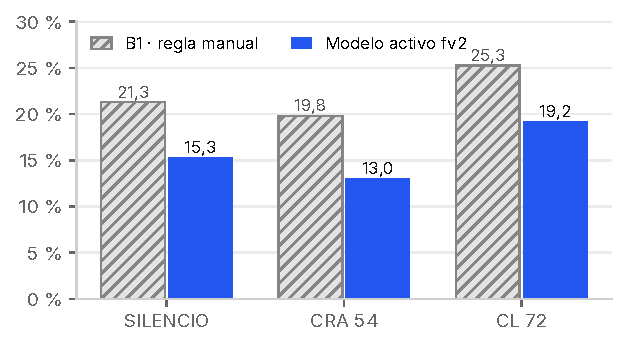
\includegraphics[width=\linewidth]{wape_rutas}\\
{\footnotesize\tenue{WAPE por ruta en la prueba reservada.}}
\end{minipage}\hfill
\begin{minipage}[t]{0.49\linewidth}\centering
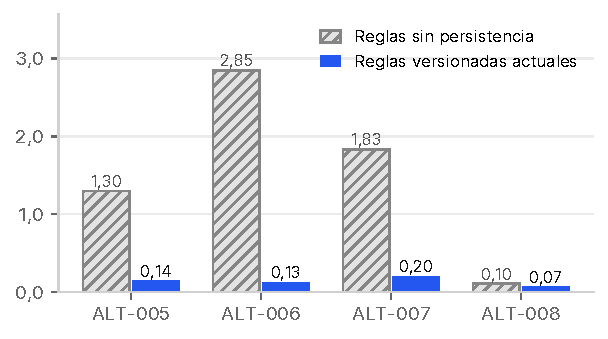
\includegraphics[width=\linewidth]{alertas_por_ruta_dia}\\
{\footnotesize\tenue{Alertas observadas por ruta y día, backtest \AlertasDesde{} a \AlertasHasta.}}
\end{minipage}
\caption{Modelo frente a la regla manual por ruta (izquierda) y volumen de alertas antes y después de la persistencia y
los episodios (derecha).}
\label{fig:rutas}
\fuente{api_frecuencias/docs/evidencias/modelo/evaluacion_modelo.json};
\evid{api_frecuencias/docs/evidencias/alertas/backtest_alertas.json}
\end{figure}

\paragraph{Incertidumbre y calibración} La banda P10--P90 del modelo cubre el \CobModelo~\% de las horas de la prueba
(objetivo 80~\%). Encima va una calibración conformal versionada: la vigente (v2) usa un cuantil por bloque horario,
ajustado solo con la validación y guardado junto al modelo con su SHA-256; en la validación baja la peor desviación de
la cobertura por grupo a \CalibPeorDesv{} puntos. En la prueba reservada cubre el \CobVdos~\% (\BajoPdiezVdos~\% bajo
el P10 y \SobrePnoventaVdos~\% sobre el P90) con una banda más angosta que la v1 (conformal móvil por ruta con días
anteriores, \CobVuno~\%), que queda como respaldo. Las horas de 18 a 20 y los días especiales de fin de año quedan bajo
el 80~\% con cualquier banda; por eso el monitoreo vigila la cobertura móvil. Cada predicción guarda el punto, P10 y
P90 calibrados, P10 y P90 del modelo, el ajuste aplicado y la versión de la calibración.
\evid{api_frecuencias/docs/evidencias/modelo/calibracion_condicional.json}

\paragraph{Explicabilidad (§9.4, RF-015)} SHAP con TreeExplainer da la explicación local de cada pronóstico; en la
escala multiplicativa del enlace Poisson, base × producto de factores reconstruye el pronóstico con error menor que
$10^{-6}$. \texttt{GET /models/\{id\}/importance} da la importancia global (permutación y media de |SHAP|), y la
respuesta de \texttt{POST /predictions/run} trae las claves de §12.3 con \texttt{explanation}.
\evid{api_frecuencias/docs/evidencias/modelo/explicacion_local_y_bandas.json}

\paragraph{Trazabilidad (§9.2)} Cada predicción guarda \texttt{model\_id}, \texttt{feature\_version},
\texttt{data\_cutoff}, \texttt{generated\_at}, horizonte y latencia; \texttt{feature\_snapshot} guarda la foto exacta de
variables por predicción, por ruta y hora. Limitación: el sentido y el segmento quedan nulos en esa foto, porque el
pronóstico por segmento y sentido (\texttt{GET /predictions/segmentos}) es un reparto proporcional del de la ruta, no
un modelo propio. El artefacto se carga una vez y se verifica su SHA-256 contra el registro; el entrenamiento es
reproducible (mismo SHA-256 en dos corridas, \path{.../modelo/entrenamiento_fv2.json}).

\paragraph{ONNX} \path{scripts/exportar_onnx.py} exporta punto, P10 y P90; \texttt{MOTOR\_INFERENCIA=onnx} los usa.
Paridad con scikit-learn: diferencia máxima de \OnnxDifMax{} pasajeros y \OnnxMsFila{} ms por fila frente a
\SklearnMsFila{} ms. \evid{api_frecuencias/docs/evidencias/monitoreo/onnx_paridad.json}

\paragraph{Monitoreo y reentrenamiento (§9.4, §9.5, RF-018, RF-019)} Cada ejecución mide en 28 días el WAPE, el MAE y
el sesgo móviles, la cobertura, el PSI de 8 variables, el volumen de predicciones y el \% de alertas descartadas
(\texttt{GET /monitoring}). La política (\path{app/servicios/politica.py}) reentrena por periodicidad, degradación (3
ejecuciones seguidas sobre \texttt{wape\_max}), deriva o cobertura; el candidato predice 14 días en sombra y solo se
activa si su WAPE es menor o igual que el del activo y que \texttt{wape\_max}, su cobertura está entre 75 y 90~\% y su
|sesgo| no pasa del 5~\%. La activación manual (\texttt{POST /models/\{id\}/activate}, admin) aplica la misma compuerta
en una ventana posterior a todo lo que vio el candidato (corte más 61 días de validación; si no, 422); saltarla exige
\texttt{forzar=true} con motivo. La activación queda auditada y se revierte sola si el modelo se degrada en sus primeros
7 días. Ejemplo real de la compuerta (sombra del \GateVentana, fuera de la prueba reservada): el candidato
\GateCandidato{} sacó \GateWAPECand~\% frente a \GateWAPEAct~\% del activo y fue \GateDecision.
\evid{api_frecuencias/docs/evidencias/monitoreo/compuerta_ejemplo.json}

% ------------------------------------------------------------------------------------------------------------------
\section{Optimización de frecuencia (§10)}
\label{sec:optimizacion}
Para cada ruta y hora, \texttt{POST /recommendations/calculate} y el ciclo diario resuelven
\[
\min_{k,\,n_t}\; \alpha\,C_{\text{op}}(n) + \beta\,E(k) + \gamma\,P_{\text{sobre}}(n) + \delta\,|k-k_{\text{prog}}|
\]
en COP por hora, donde $k=\sum_t n_t$ son los buses por hora repartidos entre tipologías $t$; $C_{\text{op}}$ suma
costo por bus-hora y por km del ciclo; $E$ es la espera media $\tfrac{60}{2k}(1+cv^2)$ valorada por pasajero;
$P_{\text{sobre}}$ es la sobrecarga esperada sobre la ocupación crítica, con la carga crítica lognormal de mediana igual al
pronóstico y dispersión tomada del P90 calibrado; y la desviación penaliza el cambio frente a la frecuencia programada.
Restricciones: headway mínimo gobernado y headway máximo efectivo, el menor entre \texttt{headway\_maximo\_min} y dos
veces \texttt{espera\_max\_min} (S12); capacidad efectiva (capacidad × ocupación objetivo) mayor o igual que el cuantil
del nivel de servicio (0,90 = P90); vehículos $\sum_t \lceil \text{ciclo}\cdot n_t/60\rceil \le$ flota; y flota por
tipología. Se resuelve como MILP con PuLP/CBC: una binaria por nivel $k$ y cortes tangentes de la sobrecarga, que es
convexa, en todas las capacidades alcanzables, así que el modelo es exacto; coincide con la enumeración exacta en
\FranjasMilpIgual{} de \FranjasTotal{} franjas reales.
\evid{api_frecuencias/docs/evidencias/optimizacion/sensibilidad.md}

\begin{itemize}
\item \textbf{Fórmulas de §10.3.} Buses por hora = techo(demanda / capacidad efectiva), headway = 60 / buses y
  vehículos = techo(ciclo / headway) salen al lado como línea base, con las restricciones, su holgura y los límites
  que mandan.
\item \textbf{Viabilidad (§18).} Si nada cumple el nivel de servicio dentro de la flota, la respuesta dice
  \texttt{viable=false} con el motivo y las cifras, y propone la mejor aproximación ejecutable, que nunca viola una
  restricción dura. En las franjas reales, \FranjasViables{} de \FranjasTotal{} son viables; no lo son
  \FranjasNoViables, donde el P90 de la demanda no cabe en la flota disponible. En el backtest del ciclo diario
  (recomendación de franja a las 6~h, \DiasRuta{} días-ruta) es viable el \ViablesBacktest~\% de las recomendaciones;
  las demás salen con su motivo, y la flota y el ciclo que las limitan son medianas de 2025 que Extreme debe confirmar
  (§19, H13).
  \evid{api_frecuencias/docs/evidencias/optimizacion/ejemplo_calculate_no_viable.json},
  \evid{.../alertas/backtest_alertas_pronostico.md}
\item \textbf{Tipologías (§10.1).} T1 $\le$ 47, T2 48--52, T3 53--62 y T4 $\ge$ 63 puestos; el MILP pone los buses
  grandes en el pico y el ajuste local de capacidad (\texttt{PUT /catalogos/capacidad}, admin, versionado) manda sobre
  el catálogo.
\item \textbf{Escenarios (RF-008).} \texttt{comparacion\_actual} compara la frecuencia programada con la recomendada en
  costo, espera, sobreocupación y vehículos; \texttt{escenario} cambia demanda, pesos, nivel de servicio, flota,
  capacidad, ciclo o headway; \texttt{sensibilidad} hace 23 variaciones de un parámetro a la vez.
\item \textbf{Plan del día (D5).} El mismo MILP reparte las salidas de 4 a 20~h con el pronóstico horario del
  modelo activo (P10, P50 y P90 de \texttt{inferencia.predecir} con $h = 60$ al inicio de cada hora) para cualquier
  fecha con variables; el pronóstico precalculado del experimento 12 del informe queda solo como opción
  (\texttt{MODELO\_PLAN=E12}). Cada hora trae límites activos, demanda de diseño, margen, \texttt{viable} y motivo, y
  la trazabilidad nombra el modelo, la calibración y la fuente del pronóstico. El ciclo diario lo deja calculado para
  el día siguiente y \texttt{GET /recommendations/plan} lo lee; sin plan para esa fecha responde 404
  \texttt{sin\_calcular}. Ejemplo (\RespEjRuta, \RespuestaFecha): \RespEjSalidas{} salidas frente a
  \RespEjProgramadas{} programadas; \RespEjNoViables.
  \evid{api_frecuencias/docs/evidencias/respuesta/respuesta_reto.md}
\item \textbf{Elasticidad.} La elasticidad de los pasajeros a las salidas (la β del informe, distinta del peso β de la
  función objetivo) está estimada en ≈~0,70 por observación (informe académico, §4.2), sin validar en campo;
  el plan usa 0,5 por prudencia; la sensibilidad está en
  \path{api_frecuencias/docs/evidencias/optimizacion/sensibilidad.md} y el piloto la mide
  (\path{PLAN_EVOLUCION.md}, §6).
\end{itemize}

% ------------------------------------------------------------------------------------------------------------------
\section{Alertas (§5)}
\label{sec:alertas}
\begin{table}[ht]
\centering\small
\caption{Catálogo de §5.2 implementado en \texttt{app/servicios/alertas.py}. Umbrales de la versión vigente de
\texttt{threshold\_config}.}
\label{tab:alertas}
\begin{tabularx}{\linewidth}{@{}l>{\raggedright\arraybackslash}p{2.6cm}X>{\raggedright\arraybackslash}p{1.9cm}@{}}
\toprule
Código & Alerta & Regla y umbral & Severidad \\
\midrule
ALT-001 & Alta demanda prevista & P90 del pronóstico $>$ capacidad disponible (buses/h × puestos); crítica si también el punto la supera; probabilidad con la banda calibrada & preventiva o crítica \\
ALT-002 & Sobreocupación & ocupación esperada u observada $\ge$ \texttt{ocupacion\_critica} (\UOcupCritica) & crítica \\
ALT-003 & Frecuencia insuficiente & buses/h actuales $<$ recomendados por el optimizador & preventiva \\
ALT-004 & Frecuencia excesiva & ocupación prevista $<$ \texttt{baja\_utilizacion} (\UBajaUtil) y la oferta supera la mínima recomendada & informativa \\
ALT-005 & Caída anormal & real $<$ \UUnoMenosCaida{} × esperado (\texttt{caida\_demanda} \UCaida) y bajo el P10 calibrado, \UPersistencia{} horas seguidas (\texttt{persistencia\_horas}) & preventiva \\
ALT-006 & Despacho ausente o tardío & minutos sin despacho $>$ headway programado + tolerancia (\UTolDespacho{} min o \texttt{Procesos.toleranciatiempo}), o déficit de salidas $>$ \UTolSalidasPct~\%, \UPersistencia{} horas & crítica \\
ALT-007 & Desviación del pronóstico & real fuera de [P10, P90] con error $\ge$ \texttt{error\_pronostico} (\UErrorPron), mismo sentido \UPersistencia{} horas & preventiva \\
ALT-008 & Consolidado anómalo & |z robusto| $\ge$ \UZ{} en subidas o viajes frente al mismo tipo de día de \USemanasRef{} semanas & preventiva \\
ALT-009 & Datos incompletos & sin datos durante \UAtraso{} períodos de ingesta, campos obligatorios faltantes u horas sin registro & crítica \\
ALT-010 & Modelo degradado & WAPE móvil de 28 días $>$ \texttt{wape\_max} (\UWapeMax) & crítica \\
\bottomrule
\end{tabularx}
\fuente{api_frecuencias/docs/evidencias/alertas/README.md}; umbrales:
\evid{api_frecuencias/docs/evidencias/alertas/backtest_alertas.json} (\texttt{umbrales\_por\_defecto})
\end{table}

\paragraph{Estructura de §5.3} \texttt{ai\_frecuencias.alert} guarda identificador y código; empresa, ruta, sentido,
viaje, conductor (solo un seudónimo HMAC, con CHECK en la base) y vehículo; detección, ventana y horizonte; severidad,
estado, observado, esperado y umbral en las mismas unidades; probabilidad o puntaje con su método; explicación en
lenguaje operativo y variables influyentes (SHAP); tendencia y serie reciente (§9.4); recomendación, asignado,
comentarios y ubicación \texttt{geography(Point,4326)} con índice GiST; el estado solo puede ser nueva, reconocida,
asignada, cerrada o descartada (CHECK en la base). La bitácora \texttt{alert\_history} guarda \emph{crear, reconocer,
asignar, comentar, cerrar, descartar}, \emph{redetección} y \emph{escalar} (RF-011): si un episodio se redetecta con
mayor severidad, la alerta sube de severidad sin cambiar de estado y se notifica si pasa a crítica; nunca baja sola, y
una redetección menos grave solo suma una ocurrencia.

\paragraph{Sin alertas excesivas (§18)} Las horas que cumplen una regla se agrupan en episodios: una alerta por episodio
y no por hora; si el episodio sigue, la ejecución siguiente actualiza la misma alerta (índice único de deduplicación
sobre las abiertas). En el backtest fuera de muestra (\DiasRuta{} días-ruta) las alertas observadas de ALT-005 a
ALT-009 bajan de \AlertasAntes{} a \AlertasAhora{} por ruta y día (con ALT-002 observada y las rupturas de RF-009,
\AlertasObsTodas), y la precisión aproximada sube: lift de \LiftAntesCinco{} a
\LiftCinco{} en ALT-005, de \LiftAntesSeis{} a \LiftSeis{} en ALT-006, de \LiftAntesSiete{} a \LiftSiete{} en ALT-007 y
de \LiftAntesOcho{} a \LiftOcho{} en ALT-008. Con el modelo de corte 2024 el resultado se repite
(\AlertasAntesDosmil{} → \AlertasAhoraDosmil). Las alertas de pronóstico del ciclo diario (una por franja) suman
\AlertasPronostico{} por ruta y día (ALT-001 \AlertasPronUno, ALT-002 \AlertasPronDos, ALT-003 \AlertasPronTres{} y
ALT-004 \AlertasPronCuatro), así que, sumadas a todas las observadas, el despachador ve \AlertasTotal{} alertas por
ruta y día.
\evid{api_frecuencias/docs/evidencias/alertas/backtest_alertas_pronostico.md} \textbf{Etiquetas (§18):} sin incidentes
etiquetados por Extreme, una muestra de alertas se revisó dos veces (\RevisionDoble); los revisores fueron
automatizados y falta la validación del área operativa de Sobusa.
\evid{api_frecuencias/docs/evidencias/alertas/revision_doble/} \textbf{Notificación (RF-012):}
adaptadores de correo y WhatsApp configurables, simulados, con circuit breaker propio.

% ------------------------------------------------------------------------------------------------------------------
\section{Base de datos (§8)}
\label{sec:bd}
Todo lo nuevo vive en el esquema \texttt{ai\_frecuencias}, creado y versionado con Alembic
(\path{alembic/versions/}, migraciones 0001 a 0006); las migraciones bajan y suben limpias en el CI (\texttt{upgrade}
→ \texttt{downgrade base} → \texttt{upgrade}). Los instantes son \texttt{TIMESTAMPTZ} guardados en UTC y presentados en America/Bogota (§8.1).

\begin{table}[ht]
\centering\small
\caption{Tablas de \texttt{ai\_frecuencias} e índices principales.}
\begin{tabularx}{\linewidth}{@{}>{\raggedright\arraybackslash}p{3.3cm}X>{\raggedright\arraybackslash}p{4.6cm}@{}}
\toprule
Tabla & Contenido & Índices y restricciones \\
\midrule
\path{model_registry} & versiones, métricas, hash, corte, auditoría de activación & único parcial: un solo activo \\
\path{prediction} & punto, P10/P90 calibrados y del modelo, ajuste, explicación local, trazabilidad & ruta-fecha, generada, \texttt{idruta} \\
\path{recommendation} & headway, buses/h, vehículos, viabilidad, objetivo, versión de umbrales; origen \texttt{franja} o \texttt{plan\_dia} & ruta-fecha; únicas por ejecución y predicción, y por ejecución, ruta, fecha y hora del plan \\
\path{respuesta_reto} & foto de la respuesta de §20 con modelo, calibración, umbrales, ejecución y fuente del pronóstico & única fecha-ruta-modelo-umbrales; fecha descendente \\
\path{alert}, \path{alert_history} & estructura de §5.3 y bitácora (con escalamiento) & CHECK de estado, ruta-fecha, código-ruta-ventana, viaje-detección, deduplicación única de abiertas, GiST en \texttt{ubicacion} \\
\path{execution_log}, \path{execution_attempt} & ejecuciones (cola, progreso, marca, métricas, \texttt{traceparent}) e intentos & estado, en cola, corriendo, única por franja programada \\
\path{data_quality_error} & errores por lote, fila, llave y causa, con valor y si bloquea & por ejecución \\
\path{demanda_observada} & histórico analítico validado & única ruta-fecha-hora (idempotencia) \\
\path{threshold_config} & umbrales y pesos versionados, con quién los aprobó y cuándo & único vigente por nombre \\
\path{model_monitoring} & monitoreo por ejecución y modelo (activo o sombra) & única por ejecución y modelo \\
\path{feature_snapshot} & foto de variables por predicción & \textbf{particionada por mes}; ejecución, predicción, ruta-fecha \\
\path{notification_log} & envíos de notificaciones & por alerta \\
\bottomrule
\end{tabularx}
\end{table}

\textbf{Dimensiones de §8.3.} \texttt{prediction}, \texttt{recommendation}, \texttt{alert},
\texttt{demanda\_observada} y \texttt{feature\_snapshot} guardan \texttt{idruta}, \texttt{idempresa}, \texttt{idproceso},
\texttt{id\_dia\_semana} (ISO 1--7) e \texttt{id\_estacionalidad}; el mapeo sale del catálogo empaquetado
(\path{datos/catalogo_rutas.json}) o de la réplica en modo integrado, y la estacionalidad queda nula porque para Sobusa
\texttt{estacionalidades\_anio} no trae filas propias (H1). La migración \path{0006_dimensiones_calidad_respuesta.py} rellena
las filas existentes y su \texttt{downgrade} está probado
(\path{tests/integracion/test_api_integracion.py::test_migracion_0006_dimensiones_sube_baja_y_rellena}).

\textbf{Particionamiento (§8.1).} \texttt{feature\_snapshot} es la tabla que más crecería: hoy guarda unas 20 filas por
ejecución (3 rutas, 3 horizontes y 1 a 3 horas), pero con variables por segmento, sentido y hora y ejecuciones horarias
llegaría a unos 17 millones de filas por ruta y año (proyección condicionada a implementar las variables por segmento;
cálculo en \path{alembic/versions/0004_monitoreo_y_trazabilidad.py}). Por eso ya va con \texttt{PARTITION BY RANGE
(ventana\_inicio)} por mes, con una función que crea la partición que falte; la retención se hace con
\texttt{DETACH/DROP PARTITION}. \textbf{Semillas:} la
migración inicial siembra la primera versión de los umbrales de §5.1; el registro de modelos se siembra con el modelo
empaquetado si está vacío. \textbf{Extensiones:} PostGIS 3.4 (\texttt{geography} + GiST); \texttt{pg\_stat\_statements}
se recomienda para el diagnóstico.

% ------------------------------------------------------------------------------------------------------------------
\section{Integración con tablas y triggers existentes (§11)}
\label{sec:integracion}
La integración se probó en una réplica local (PostgreSQL 14 + PostGIS) creada con los ocho scripts de Extreme (SHA-256
verificados) y cargada con las exportaciones: 3.379.899 filas, 14 llaves foráneas sin huérfanos, las cuatro funciones y
el trigger \texttt{tg\_timbrada\_segmento} sobre \texttt{conteo\_pasajeros} activos. Dos correcciones mínimas de los
scripts (E1 y E2) y un hallazgo (H1) quedan documentados.
\evid{api_frecuencias/docs/evidencias/replica/replica_init.log}, \evid{.../replica/replica_errata.txt}

\begin{itemize}
\item \textbf{Llegada real por el trigger.} 584 eventos crudos de tres viajes reservados, insertados uno a uno como
  los insertaría la captura, pasan por el trigger (50,2 ms por fila) y dejan 228 filas en \texttt{timbradas\_segmentos},
  iguales a la exportación (223 de 223 pares; Σ subidas 201 = 201). La API, en modo integrado, relee 1.263 franjas en
  la ventana de solape, entrega exactamente 1 y descarta 1.262; sin datos nuevos, lee 0.
  \evid{api_frecuencias/docs/evidencias/replica/replica_llegada.txt}
\item \textbf{Funciones de Extreme.} \path{fn_insert_timbradas_anio} devuelve TRUE en 3 de 3 viajes y
  \path{fn_consolidar_timbradas_historicas} resella las 10.731 filas del consolidado; el lector con huella entrega
  solo las 7.952 que cambiaron (H7).
\end{itemize}

\begin{table}[ht]
\centering\small
\caption{\texttt{EXPLAIN (ANALYZE, BUFFERS)} como \texttt{lector\_ia}, antes y después de la propuesta de índices
(\texttt{propuesta\_indices.sql}, aplicada por el DBA solo en la réplica y retirada al terminar).}
\begin{tabularx}{\linewidth}{@{}Xll@{}}
\toprule
Consulta & Ejecución sin novedades & Bloque grande de llegada \\
\midrule
\path{timbradas_segmentos} por marca & 239 ms (Seq Scan) → 0,01 ms (Index Scan) & 500.000 filas: 454 → 245 ms \\
\path{demanda_segmentos} (ciclo) & 269 → 0,07 ms & 1.262 franjas: 5,26 → 5,03 s \\
\path{timbradas_consolidado} & 1,6 → 0,01 ms & 10.731 filas: 6,1 → 4,3 ms \\
\path{timbradas_anio} & 4,9 → 0,01 ms & 22.542 filas: 17,0 → 4,8 ms \\
\bottomrule
\end{tabularx}
\fuente{api_frecuencias/docs/evidencias/replica/explain_incremental.txt}. Una ejecución diaria lee el 0,085~\% de la
tabla.
\end{table}

\begin{table}[ht]
\centering\small
\caption{Controles de no interferencia de §11.3 y su prueba automática (\texttt{tests/replica}).}
\begin{tabularx}{\linewidth}{@{}>{\raggedright\arraybackslash}p{4.4cm}X@{}}
\toprule
Control & Cómo se cumple y qué lo prueba \\
\midrule
Usuario técnico con SELECT & \texttt{lector\_ia}: solo \texttt{GRANT SELECT}; sus \NIntentosLector{} intentos de escritura (16 tipos, dos modos de sesión) fallan con 25006 o 42501 \\
Usuario que escribe solo en \texttt{ai\_frecuencias} & \texttt{escritor\_ia}, dueño del esquema; \NIntentosEscritor{} intentos de escribir o alterar 14 tablas de Extreme dan 42501 (en total, \NIntentosTotal{} intentos y 0 escrituras indebidas) \\
READ ONLY con timeout & la fuente abre \texttt{READ ONLY} + \texttt{statement\_timeout} + zona horaria y termina con ROLLBACK; el rol tiene los mismos valores por omisión \\
Ningún DDL operacional & ni ALTER, ni CREATE INDEX, ni DROP, ni LOCK en \texttt{public} para ninguno de los dos \\
No deshabilitar triggers & \texttt{DISABLE TRIGGER} y \texttt{DROP TRIGGER} fallan; el trigger sigue con \texttt{tgenabled = 'O'} \\
No modificar funciones ni índices & \texttt{CREATE OR REPLACE FUNCTION} falla; los índices son una propuesta para el DBA \\
Consultas pesadas en réplica & todo lo medido corre en la réplica local; la base compartida del reto no se usa \\
\bottomrule
\end{tabularx}
{\footnotesize\color{rol-tinta-3}Fuente: los intentos son casos de \path{tests/replica/test_roles.py} y
\path{test_integrado.py} en \FuenteIntentos; la corrida manual por script está en
\path{api_frecuencias/docs/evidencias/replica/replica_roles.txt}.}
\end{table}

% ------------------------------------------------------------------------------------------------------------------
\section{API REST (§12)}
\label{sec:api}
\textbf{Convenciones (§12.1).} Ruta base \texttt{/api/v1} (versionada en la ruta); JSON UTF-8; instantes ISO-8601 con
zona (-05:00); validación con Pydantic; error uniforme
\path|{"error": {"codigo", "mensaje", "detalle", "correlation_id"}}| también para el 422; colecciones con
\texttt{limite} (1 a 500), \texttt{desplazamiento}, \texttt{orden} (prefijo «-» descendente, lista blanca de campos) y
filtros; exportaciones CSV y XLSX de lo filtrado (RF-017); cabecera \texttt{X-Correlation-Id} en cada respuesta;
Swagger UI y \texttt{/openapi.json} solo fuera de producción (\texttt{ENTORNO}). \textbf{Seguridad:} cabecera
\texttt{X-API-Key} con tres roles (operador lee y gestiona alertas; analista además ejecuta, calcula y entrena; admin
además activa, revierte y cambia umbrales y capacidad); las claves se guardan solo como hash SHA-256 y la auditoría usa
el usuario autenticado, no el que diga el cuerpo. Sin clave: 401 con \texttt{WWW-Authenticate}; rol insuficiente: 403
con el rol exigido. \evid{api_frecuencias/docs/evidencias/seguridad/matriz_roles.txt}

\textbf{Endpoints.} La tabla se genera desde \OrigenTablaAPI{} (\NOperaciones{} operaciones, \NOperacionesVuno{} bajo
\texttt{/api/v1} y las demás en la raíz); los diez de §12.2 están todos y Schemathesis los recorre en
\path{tests/contrato}. Los procesos largos no corren dentro de la petición (§7.1): \texttt{POST /frequency/executions},
\texttt{POST /models/train} y \texttt{POST /respuesta/calcular} encolan y responden 202 con el \texttt{execution\_id};
\texttt{GET /respuesta} y \texttt{GET /recommendations/plan} leen lo ya calculado.

{\footnotesize
\setlength{\LTpre}{2pt}\setlength{\LTpost}{2pt}
% Generado por documentos/tabla_api.py desde la aplicación FastAPI (app.main): 62 operaciones. No editar a mano.
\begin{longtable}{@{}l>{\raggedright\arraybackslash}p{5.3cm}l>{\raggedright\arraybackslash}p{7.2cm}@{}}
\toprule Método & Ruta (bajo \texttt{/api/v1}) & Rol mínimo & Finalidad \\ \midrule \endhead
\bottomrule \endfoot
\texttt{POST} & \path{/frequency/executions} & analista & Ejecutar lectura incremental, predicción y optimización (job en segundo plano) \\
\texttt{GET} & \path{/frequency/executions} & operador & Listar ejecuciones \\
\texttt{GET} & \path{/frequency/executions/{execution_id}} & operador & Corte, estado, métricas y errores \\
\texttt{GET} & \path{/frequency/executions/{execution_id}/errors} & operador & Errores de calidad de la ejecución por lote, fila, llave y causa \\
\texttt{GET} & \path{/predictions/segmentos} & operador & Pronóstico por segmento y sentido (desagregación documentada del pronóstico de la ruta) \\
\texttt{POST} & \path{/predictions/run} & analista & Inferencia para una ruta y un horizonte (incluye la recomendación derivada) \\
\texttt{GET} & \path{/predictions} & operador & Consultar pronósticos por filtros \\
\texttt{GET} & \path{/predictions/export} & operador & Exportar pronósticos filtrados (CSV o XLSX) \\
\texttt{GET} & \path{/predictions/{prediction_id}} & operador & Una predicción \\
\texttt{POST} & \path{/recommendations/calculate} & analista & Calcular frecuencia y flota con la función objetivo de §10.2, tipologías, escenarios y… \\
\texttt{GET} & \path{/recommendations/plan} & operador & Plan del día por hora con el modelo activo (salidas, headway, vehículos, viabilidad y costo) \\
\texttt{GET} & \path{/recommendations} & operador & Consultar recomendaciones \\
\texttt{GET} & \path{/recommendations/export} & operador & Exportar recomendaciones filtradas (CSV o XLSX) \\
\texttt{GET} & \path{/alerts} & operador & Listar alertas por estado, nivel, ruta, fecha y lugar \\
\texttt{GET} & \path{/alerts/export} & operador & Exportar alertas filtradas (CSV o XLSX) \\
\texttt{GET} & \path{/alerts/{alert_id}} & operador & Una alerta \\
\texttt{PATCH} & \path{/alerts/{alert_id}/status} & operador & Reconocer, asignar, comentar, cerrar o descartar (queda en la bitácora) \\
\texttt{GET} & \path{/alerts/{alert_id}/history} & operador & Bitácora de cambios de la alerta \\
\texttt{GET} & \path{/models} & operador & Consultar el registro de modelos \\
\texttt{POST} & \path{/models/train} & analista & Entrenar un modelo candidato con los datos validados hasta una fecha (job) \\
\texttt{POST} & \path{/models/rollback} & admin & Revertir al modelo activo anterior \\
\texttt{GET} & \path{/models/{model_id}} & operador & Ficha de un modelo \\
\texttt{POST} & \path{/models/{model_id}/activate} & admin & Activar una versión con la compuerta de cuatro criterios, en una ventana posterior a todo… \\
\texttt{GET} & \path{/models/{model_id}/evaluation} & operador & Evaluación del modelo: la registrada y, con desde/hasta, la de una ventana sobre datos… \\
\texttt{GET} & \path{/models/{model_id}/importance} & operador & Importancia global: permutación (aumento del MAE) y media de |SHAP| \\
\texttt{GET} & \path{/thresholds} & operador & Umbrales vigentes, su versión y si están aprobados \\
\texttt{PUT} & \path{/thresholds} & admin & Cambiar umbrales: crea una versión nueva del conjunto \\
\texttt{GET} & \path{/thresholds/history} & operador & Histórico de versiones de los umbrales \\
\texttt{POST} & \path{/thresholds/{version}/aprobar} & admin & Aprobar una versión de umbrales (validación del área operativa, §5.1) \\
\texttt{GET} & \path{/scheduler} & operador & Planificador interno: próximas ejecuciones, últimas franjas encoladas y estado de la cola \\
\texttt{GET} & \path{/catalogos} & operador & Catálogos disponibles y fuente configurada \\
\texttt{GET} & \path{/catalogos/procesos} & operador & Procesos (empresa operadora) \\
\texttt{GET} & \path{/catalogos/procesos/export} & operador & Exportar procesos (CSV o XLSX) \\
\texttt{GET} & \path{/catalogos/empresas} & operador & Empresas por proceso \\
\texttt{GET} & \path{/catalogos/empresas/export} & operador & Exportar empresas (CSV o XLSX) \\
\texttt{GET} & \path{/catalogos/rutas} & operador & Rutas: frecuencia vigente, capacidad (y cap\_min/cap\_max si existen), ciclo y flota \\
\texttt{GET} & \path{/catalogos/rutas/export} & operador & Exportar rutas (CSV o XLSX) \\
\texttt{GET} & \path{/catalogos/rutas/{idruta}} & operador & Una ruta con sus parámetros por hora \\
\texttt{GET} & \path{/catalogos/segmentos} & operador & Segmentos de ruta (rutas\_segmentos) con longitud y geometría GeoJSON \\
\texttt{GET} & \path{/catalogos/segmentos/export} & operador & Exportar segmentos (CSV o XLSX; geometría simplificada como GeoJSON) \\
\texttt{GET} & \path{/catalogos/vehiculos} & operador & Vehículos: capacidad sentados + de pie y tipología (sin placa, conductor ni propietario) \\
\texttt{GET} & \path{/catalogos/vehiculos/export} & operador & Exportar vehículos (CSV o XLSX) \\
\texttt{GET} & \path{/catalogos/vehiculos/tipologias} & operador & Capacidad por ruta y tipología (vehículos, mediana, mínimo y máximo) \\
\texttt{GET} & \path{/catalogos/viajes} & operador & Programación de viajes (idprogramacion, ruta, hora programada y vehículo) \\
\texttt{GET} & \path{/catalogos/viajes/export} & operador & Exportar viajes filtrados (CSV o XLSX) \\
\texttt{GET} & \path{/catalogos/despachos} & operador & Despachos reales: salida y llegada, retraso frente a la hora programada \\
\texttt{GET} & \path{/catalogos/despachos/export} & operador & Exportar despachos filtrados (CSV o XLSX) \\
\texttt{GET} & \path{/catalogos/capacidad} & operador & Capacidad vigente por ruta (catálogo o ajuste local) y ajustes por tipología \\
\texttt{PUT} & \path{/catalogos/capacidad} & admin & Ajustar la capacidad operativa de una ruta o tipología (admin; versión nueva y auditada) \\
\texttt{GET} & \path{/catalogos/capacidad/historial} & operador & Historial de ajustes de capacidad (versión, acción, valor anterior y nuevo, quién y por qué) \\
\texttt{GET} & \path{/monitoring} & operador & Monitoreo por ejecución: deriva (PSI), error móvil, cobertura, volumen y alertas descartadas \\
\texttt{GET} & \path{/monitoring/export} & operador & Exportar el monitoreo filtrado (CSV o XLSX) \\
\texttt{GET} & \path{/monitoring/policy} & operador & Política de aprendizaje continuo: ¿reentrenar?, retadores en sombra y umbrales \\
\texttt{GET} & \path{/monitoring/feature-snapshots} & operador & Foto de variables (§11.2) por ejecución, predicción o ruta, con fecha de corte y versión \\
\texttt{GET} & \path{/segmentos/estadisticas} & operador & Promedio, máximo y mínimo de subidas, bajadas y pasajeros por segmento, estacionalidad,… \\
\texttt{GET} & \path{/segmentos/estadisticas/export} & operador & Exportar las estadísticas por segmento (CSV o XLSX) \\
\texttt{GET} & \path{/segmentos/zonas} & operador & Demanda por zona tarifaria (timbradas\_anio\_zonas / timbradas\_consolidado\_zonas) \\
\texttt{GET} & \path{/respuesta} & operador & Respuesta a la pregunta final del reto (§20) \\
\texttt{POST} & \path{/respuesta/calcular} & analista & Calcular la respuesta del reto para una fecha (job en la cola, rol analista) \\
\texttt{GET} & \path{/respuesta/export} & operador & Exportar la respuesta del reto por ruta y hora (CSV o XLSX) \\
\midrule
\multicolumn{4}{@{}l}{\emph{En la raíz del servidor, fuera de \texttt{/api/v1} (ruta absoluta)}} \\
\texttt{GET} & \path{/health} & pública & Estado del servicio y de la base \\
\texttt{GET} & \path{/metrics} & pública & Métricas Prometheus \\
\end{longtable}

}

% ------------------------------------------------------------------------------------------------------------------
\filbreak   % el título no queda solo al pie de una página si la tabla empieza en la siguiente
\section{Requisitos no funcionales (§13)}
\label{sec:rnf}
\begin{longtable}{@{}>{\raggedright\arraybackslash}p{2.5cm}>{\raggedright\arraybackslash}p{7.9cm}>{\raggedright\arraybackslash}p{5.6cm}@{}}
\caption{Cómo se cumple cada RNF y dónde está la evidencia (rutas bajo \texttt{api\_frecuencias/docs/evidencias/}).}\\
\toprule RNF & Cómo se cumple & Evidencia \\ \midrule \endfirsthead
\toprule RNF & Cómo se cumple & Evidencia \\ \midrule \endhead
\bottomrule \endfoot
001 Disponibilidad & cola en PostgreSQL con reserva y reintento; un \texttt{kill} durante la lectura o la predicción se retoma sin duplicar predicciones ni alertas (45 de 45 comprobaciones con \texttt{docker kill}) & \path{cola/caida_rnf001_docker.txt} \\
002 Rendimiento & k6: \Kpeticiones{} consultas paginadas, hasta \Kvus{} usuarios, p95 \Kpnoventaycinco{} ms y \Kerrores~\% de errores; durante una ingesta, p95 \Kingesta{} ms (límite 2.000 ms) & \path{pruebas/k6_consultas.txt}, \path{pruebas/k6_ingesta.txt} \\
003 Ingesta & \IngestaFilas{} filas con COPY + upsert en \IngestaSegundos{} s (\IngestaTasa{} filas/s), memoria pico \IngestaMemoria{} MiB & \path{rendimiento.txt}, \path{cola/ingesta.txt} \\
004 Asincronía & \texttt{POST /frequency/executions}, \texttt{/models/train} y \texttt{/respuesta/calcular} responden 202 y encolan; progreso por etapa y reintento con espera creciente & \path{cola/demo_ciclo_api_cola.txt} \\
005 Escalabilidad & API sin estado; dos réplicas reparten 20 ejecuciones 10/10 sin duplicados; procesamiento particionable por ruta y fecha & \path{cola/replicas.txt} \\
006 Observabilidad & logs JSON con \texttt{correlation\_id} y \texttt{execution\_id}; \texttt{/metrics}; una traza OpenTelemetry de 39 spans por ciclo & \path{seguridad/traza_ejecucion.json}, \path{seguridad/jaeger_resumen.txt} \\
007 Mantenibilidad & arquitectura modular; cobertura \Cobertura~\%; ruff, bandit y SonarQube & \FuenteCobertura, \path{sonarqube/resumen.md} \\
008 Portabilidad & Docker Compose con la API, PostgreSQL 14 + PostGIS y la migración; variables de entorno & \path{api_frecuencias/docker-compose.yml}, \path{docs/despliegue.md} \\
009 Compatibilidad & OpenAPI versionado; prueba de compatibilidad contra \path{docs/openapi.json}; Alembic de ida y vuelta & \path{tests/contrato}, \path{pruebas/ci_local.txt} \\
010 Resiliencia & timeout, reintento controlado y circuit breaker (3 fallos abren, semiabierto a los 60 s) en la fuente y en las notificaciones & \path{seguridad/resiliencia.txt} \\
011 Trazabilidad IA & cada salida liga datos (corte, ejecución), variables (versión y foto), regla (versión de umbrales) y modelo & \path{modelo/explicacion_local_y_bandas.json} \\
012 Accesibilidad & tablero con contraste validado por pares, navegable con teclado y estados con icono y palabra & \path{tablero/verificar_estilo_vivo_api_arriba.txt} \\
013 Calidad de código & \SonarResumen & \path{sonarqube/resumen.md} \\
014 Pruebas unitarias & \NUnit{} pruebas unitarias con pytest y \texttt{unittest.mock}, ejecutadas en el CI & \path{api_frecuencias/ci/github_actions_entrega.yml} \\
\end{longtable}

\begin{figure}[ht]
\centering
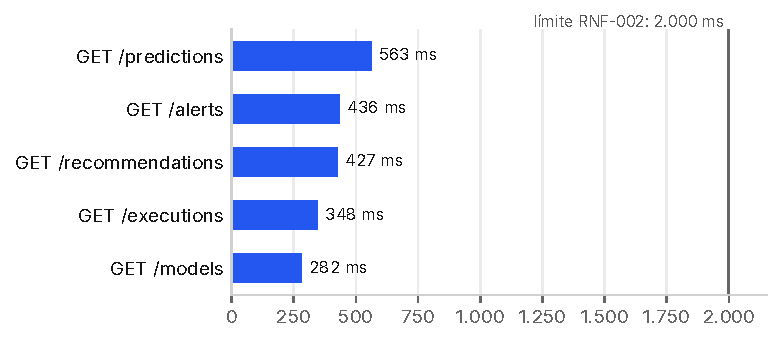
\includegraphics[width=0.62\linewidth]{k6_p95}
\caption{RNF-002: p95 por recurso con k6 (rampa hasta \Kvus{} usuarios virtuales, \Kpeticiones{} peticiones
paginadas al azar dentro del total real), frente al límite de 2 s.}
\fuente{api_frecuencias/docs/evidencias/pruebas/k6_consultas.json}
\end{figure}

% ------------------------------------------------------------------------------------------------------------------
\section{Pruebas (§14)}
\label{sec:pruebas}
\begin{minipage}[t]{0.52\linewidth}
\vspace{0pt}\small
\begin{tabularx}{\linewidth}{@{}lrX@{}}
\toprule
Nivel (§14.1) & Pruebas & Herramientas \\
\midrule
Unitarias & \NUnit & pytest, \texttt{unittest.mock} \\
Integración & \NInteg & pytest, API con base real \\
Réplica (rendimiento SQL) & \NReplica & roles, EXPLAIN, llegada \\
Contrato & \NContrato & OpenAPI, HTTPX, Schemathesis \\
Datos/ML & \NDatos & distribución, no regresión, fuga \\
Testcontainers & \NTcont & PostGIS 14 efímero, Alembic\NTcontNota \\
Carga & k6 & consultas e ingesta \\
\midrule
Total & \Ntotal & \Npasan{} aprobadas, \Nfallan{} fallidas, \Nomitidas{} omitidas \\
\bottomrule
\end{tabularx}
\end{minipage}\hfill
\begin{minipage}[t]{0.45\linewidth}
\vspace{0pt}
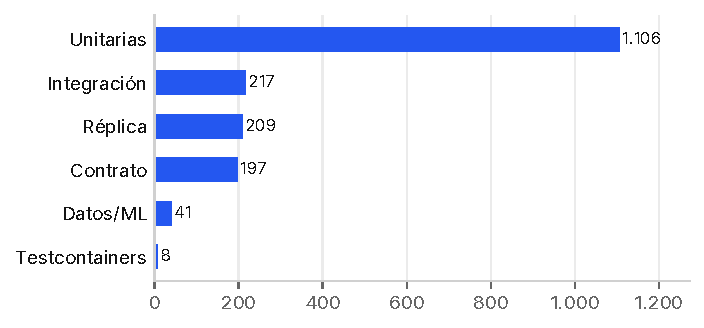
\includegraphics[width=\linewidth]{pruebas_por_nivel}
\end{minipage}

{\footnotesize\color{rol-tinta-3}Fuente: \FuentePruebas, \CorridaPruebas, con la réplica; cobertura de
\path{app/}: \FuenteCobertura.} Las omitidas lo son a propósito (la caída real con \texttt{docker kill} y las
escrituras en la réplica, que se activan con una variable). SonarQube importó \SonarPruebas{} pruebas en su análisis
(\path{api_frecuencias/docs/evidencias/sonarqube/measures.json}).

\textbf{Integración continua.} \path{api_frecuencias/ci/github_actions_entrega.yml}, el flujo de GitHub Actions:
Python 3.11 y 3.13, servicio PostGIS 14-3.4, ruff, bandit, Alembic de ida y vuelta, pytest con cobertura mínima de
85~\%, Testcontainers, verificación de deriva del OpenAPI, un trabajo de caída y uno de SonarQube. Estado: \EstadoCI.
En GitHub no hay réplica con los datos del reto, así que allí se omiten las pruebas de \path{tests/replica}.

\textbf{Criterios de §14.2 y su evidencia.} Instalación por migraciones (Testcontainers crea el esquema desde cero);
carga repetida sin duplicar y errores por lote, fila y causa (sección~\ref{sec:datos}); predicción con horizonte,
incertidumbre, versión y explicación (sección~\ref{sec:modelo}); recomendación que respeta capacidad y restricciones
(sección~\ref{sec:optimizacion}); alertas deduplicadas con historial (sección~\ref{sec:alertas}); modelo mejor que la
línea base; marca de agua sin escribir en los consolidados (sección~\ref{sec:integracion}); y el ciclo de
demostración contra la API en Docker: llega un día nuevo y se leen solo sus \DemoFilasNuevas{} filas (repetir lee
\DemoFilasRepeticion), el activo tiene un WAPE de \DemoWapeNuevo~\% sobre lo recién llegado, el candidato
\DemoCandidato{} se entrena como job, saca \DemoWapeCand~\% frente a \DemoWapeAct~\% del activo en la misma validación
temporal (\DemoVentana) y queda \DemoDecision; el ciclo completo tarda \DemoTotalSeg{} s
(\path{scripts/demo_ciclo_api.py}, \evid{api_frecuencias/docs/evidencias/despliegue/demo_ciclo_api.txt}).

% ------------------------------------------------------------------------------------------------------------------
\section{Seguridad y datos personales (§18)}
\label{sec:seguridad}
\begin{tabularx}{\linewidth}{@{}>{\raggedright\arraybackslash}p{3.5cm}X@{}}
\toprule
Riesgo & Mitigación implementada \\
\midrule
Exposición de datos & los catálogos nunca devuelven placa, conductor, propietario, contactos, módem, póliza ni GPS (0 columnas prohibidas, \path{catalogos/sin_datos_personales.txt}); el conductor de una alerta es un seudónimo HMAC-SHA256 con secreto del entorno y la base rechaza un valor en claro; las lecturas de \texttt{"Procesos"} omiten sus columnas de credenciales \\
Secretos & ninguno en el repositorio: conexión, claves y secreto del seudónimo llegan por variables de entorno (\path{.env.example} con marcadores que deben cambiarse); las claves de API se guardan como hash; el log no las imprime \\
Acceso & tres roles con mínimo privilegio; la escritura en la base de Extreme es imposible por permisos, no solo por código \\
Consulta pesada & lectura incremental, \texttt{statement\_timeout}, réplica, índices solo por el DBA y circuit breaker \\
Alertas excesivas & persistencia, episodios, deduplicación y severidades; descartadas medidas en el monitoreo \\
Recomendación inviable & estado \texttt{viable=false} con motivo y mejor aproximación \\
Deriva & PSI, error móvil, sombra, compuerta y reversión automática \\
Retención & particiones mensuales con \texttt{DETACH/DROP} en la tabla de mayor volumen \\
\bottomrule
\end{tabularx}

% ------------------------------------------------------------------------------------------------------------------
\section{Despliegue y operación (§7.1, RNF-008, E09)}
\label{sec:despliegue}
\textbf{Contenedores.} \path{api_frecuencias/docker-compose.yml} levanta \texttt{db} (PostgreSQL 14 + PostGIS 3.4),
\texttt{migrar} (Alembic \texttt{upgrade head} antes de la API) y \texttt{api} (FastAPI con su trabajador de cola y el
planificador), más \texttt{jaeger} para las trazas. Dos archivos se suman al base: \path{docker-compose.replicas.yml}
(dos réplicas de la API sobre la misma cola) y \path{docker-compose.integracion.yml} (modo integrado: la API lee de la
base de Extreme o de su réplica con \texttt{lector\_ia} y escribe con \texttt{escritor\_ia}). El perfil
\texttt{operacional} con \texttt{cargador\_replica} arma la réplica local con los scripts de Extreme. Los pasos y la
verificación están en \path{api_frecuencias/docs/despliegue.md}.

\textbf{Configuración por ambiente (§7.1).} Todo entra por variables de entorno; \path{.env.example} trae los nombres
con marcadores que deben cambiarse (por ejemplo, las contraseñas y \texttt{SEUDONIMO\_SECRETO}) y \path{.env} no se
versiona. Las principales, por grupo:
\begin{itemize}
\item \emph{Bases:} \texttt{DATABASE\_URL} (resultados), \texttt{FUENTE} y \texttt{FUENTE\_DATABASE\_URL} (lectura),
  \texttt{FUENTE\_TABLA}, \texttt{FUENTE\_SOLAPE\_MIN}, \texttt{FUENTE\_STATEMENT\_TIMEOUT\_MS},
  \texttt{CATALOGOS\_DATABASE\_URL}.
\item \emph{Ejecución:} \texttt{PLAN\_EJECUCION\_CRON} (por omisión, todos los días a las 05:15),
  \texttt{PLAN\_REENTRENAMIENTO\_CRON} (lunes a las 04:00), \texttt{TRABAJADORES}, \texttt{LEASE\_SEGUNDOS},
  \texttt{MAX\_REINTENTOS}, \texttt{MOTOR\_INFERENCIA} (\texttt{sklearn} u \texttt{onnx}).
\item \emph{Seguridad:} \texttt{AUTH\_HABILITADA}, \texttt{API\_KEYS} (solo hashes), \texttt{SEUDONIMO\_SECRETO},
  \texttt{ENTORNO} (en \texttt{produccion} se apagan Swagger y \texttt{/openapi.json}), \texttt{METRICAS\_PUBLICAS}.
\item \emph{Resiliencia y observabilidad:} \texttt{CIRCUITO\_FUENTE\_FALLOS\_MAX}, \texttt{CIRCUITO\_FUENTE\_REINICIO\_S},
  \texttt{OTEL\_EXPORTADOR}, \texttt{LOG\_NIVEL}; notificaciones con \texttt{NOTIFICACIONES\_CANALES} y sus destinatarios.
\end{itemize}

\textbf{Ciclo diario en operación.} El planificador encola una ejecución por franja (índice único: dos réplicas no
encolan dos veces la misma); el trabajador la reclama con \texttt{SKIP LOCKED}, corre las etapas con progreso
visible en \texttt{GET /frequency/executions/\{id\}} y confirma resultados, marca de agua y estado en una sola
transacción. Al cerrar calcula el plan del día siguiente y la foto de la respuesta; si eso falla, la ejecución queda
\texttt{ok} con la advertencia en sus métricas. Si la política lo pide, encola un reentrenamiento, que pasa por sombra y compuerta antes de cualquier
activación; un administrador puede activar o revertir con auditoría (\texttt{POST /models/\{id\}/activate},
\texttt{/models/rollback}). Las demostraciones del ciclo completo se reproducen con \path{scripts/demo_ciclo_api.py}.

% ------------------------------------------------------------------------------------------------------------------
\clearpage
\section{Decisiones técnicas}
\label{sec:adr}
\begin{longtable}{@{}>{\raggedright\arraybackslash}p{3.5cm}>{\raggedright\arraybackslash}p{3.6cm}>{\raggedright\arraybackslash}p{6.9cm}@{}}
\toprule Decisión & Alternativas & Razón \\ \midrule \endfirsthead
\toprule Decisión & Alternativas & Razón \\ \midrule \endhead
\bottomrule \endfoot
Adaptador propio de solo lectura con lista blanca de SELECT & ORM sobre las tablas de Extreme; vistas nuevas en su esquema & RF-002 y §11.3: ningún objeto nuevo en el esquema operacional; la guarda rechaza DML y DDL antes de conectarse \\
Marca de agua con ventana de solape y huella md5 & solo \texttt{ultima\_actualizacion > marca} & las marcas no tienen zona y llevan la hora de inicio de la transacción (H8) y el cierre resella todo (H7): sin solape se pierden filas tardías y sin huella se reprocesa todo \\
Cola de trabajos en PostgreSQL (\texttt{SKIP LOCKED}) & Celery o RQ con Redis & un servicio menos; los resultados y el «ok» de la ejecución se confirman en la misma transacción (exactamente una vez) \\
HGB Poisson con cuantiles, exportable a ONNX & LightGBM (experimento 11 del informe) o el híbrido con un modelo fundacional (experimento 12); redes temporales & reproducible desde Python con scikit-learn, sin GPU ni descargas en cada solicitud (§9.2), paridad ONNX y latencia de \OnnxMsFila{} ms por fila; el 13,94 y el 13,62~\% del informe se miden a 7 días sobre todo 2025, otra métrica que la del producto (\WAPEact~\% por ruta y hora en la prueba) \\
Calibración conformal versionada (v2 por bloque horario; v1 móvil por ruta de respaldo) & usar la banda de cuantiles tal cual & acerca la cobertura al 80~\% sin tocar el pronóstico, se ajusta solo con la validación y se verifica por hash; la banda del modelo cubría 67,67~\% en 2024 \\
MILP con PuLP/CBC & heurística; OR-Tools & exacto (verificado contra enumeración), solucionador libre y una sola formulación para la franja y para el plan del día \\
Episodios y persistencia de 2 horas & una alerta por hora & §18 «alertas excesivas»: de \AlertasAntes{} a \AlertasAhora{} alertas por ruta y día con mayor precisión \\
Umbrales y pesos en \texttt{threshold\_config} versionado & constantes en el código & regla de gobierno de §5.1: se cambian sin recompilar y cada resultado guarda la versión que usó \\
Claves de API por rol & OAuth2/JWT con un proveedor de identidad & el prototipo no tiene proveedor de identidad; la política está en un solo lugar (\path{app/seguridad.py}) y se puede cambiar por JWT sin tocar los routers \\
Partición mensual solo en \texttt{feature\_snapshot} & particionar todas las tablas & §8.1 «cuando se justifique»: es la que crecería con las variables por segmento (proyección de 17 millones de filas por ruta y año); las demás crecen unas miles de filas por día \\
Respuesta y plan calculados en la cola y leídos por el GET & resolver el MILP dentro de la petición & §7.1: un GET no corre un proceso largo; la foto guarda modelo, calibración y umbrales, y el 404 \texttt{sin\_calcular} dice cómo pedirla \\
El tablero consume la API & leer la base desde el tablero & una sola fuente de verdad, los mismos roles y la misma auditoría \\
\end{longtable}
\fuente{api_frecuencias/docs/evidencias/modelo/evaluacion_modelo.md} (cobertura de la banda del modelo en 2024) y
las secciones anteriores.

% ------------------------------------------------------------------------------------------------------------------
\section{Correspondencia con la especificación v1.5}
\label{sec:correspondencia}
\small
\begin{longtable}{@{}>{\raggedright\arraybackslash}p{3.6cm}>{\raggedright\arraybackslash}p{3.3cm}>{\raggedright\arraybackslash}p{8.9cm}@{}}
\toprule Apartado & En este documento & Evidencia principal (bajo \texttt{api\_frecuencias/docs/}) \\ \midrule \endfirsthead
\toprule Apartado & En este documento & Evidencia principal \\ \midrule \endhead
\bottomrule \endfoot
§3.1 módulos & \ref{sec:arquitectura} & tabla~\ref{tab:componentes}; \path{evidencias/catalogos/README.md} \\
§4 RF-001, RF-002, RF-014 & \ref{sec:integracion} & \path{evidencias/replica/replica_roles.txt} \\
§4 RF-003, RF-005, RF-006 & \ref{sec:modelo} & \path{evidencias/modelo/contexto_operacional.json}, \path{horizontes.json} \\
§4 RF-004, §6.3 & \ref{sec:datos} & \path{evidencias/replica/replica_llegada.txt} \\
§4 RF-007, RF-008, §10 & \ref{sec:optimizacion} & \path{evidencias/optimizacion/sensibilidad.md} \\
§4 RF-009 a RF-012, §5 & \ref{sec:alertas} & \path{evidencias/alertas/backtest_alertas.md} \\
§4 RF-013, §9.5, §11.2 & \ref{sec:datos}, \ref{sec:integracion} & \path{evidencias/despliegue/demo_ciclo_api.txt} \\
§4 RF-015, §9.4 & \ref{sec:modelo} & \path{evidencias/modelo/explicacion_local_y_bandas.json} \\
§4 RF-016, RF-017 & \ref{sec:api} & \path{evidencias/contrato/operaciones_codigos.txt} (CSV y XLSX por operación), \path{evidencias/catalogos/rendimiento_exportaciones.txt}, \path{evidencias/tablero/export_recomendaciones_dash.csv} \\
§4 RF-018, RF-019 & \ref{sec:modelo} & \path{evidencias/monitoreo/compuerta_ejemplo.json} \\
§7 arquitectura & \ref{sec:arquitectura}, \ref{sec:despliegue} & \path{evidencias/seguridad/traza_ejecucion.json} \\
§8 base de datos & \ref{sec:bd} & \path{alembic/versions/} (migraciones) \\
§9.3 evaluación & \ref{sec:modelo} & \path{evidencias/modelo/evaluacion_modelo.md} \\
§11.3 no interferencia & \ref{sec:integracion} & \path{evidencias/replica/explain_incremental.txt} \\
§12 API & \ref{sec:api} & \path{docs/openapi.json}, \path{evidencias/seguridad/matriz_roles.txt} \\
§13 RNF-001 a RNF-014 & \ref{sec:rnf} & \path{evidencias/rendimiento.txt}, \path{evidencias/cola/} \\
§14 pruebas & \ref{sec:pruebas} & \FuentePruebas, \path{evidencias/pruebas/ci_local.txt} \\
§16 calidad de código & \ref{sec:rnf} (RNF-013) & \path{evidencias/sonarqube/resumen.md} \\
§18 riesgos & \ref{sec:seguridad} & \path{evidencias/catalogos/sin_datos_personales.txt} \\
§19 información de Extreme & 1 & \path{docs/hallazgos_extreme.md} (\HallazgosRango) \\
§20 pregunta del reto & \ref{sec:optimizacion}, \ref{sec:api} & \path{evidencias/respuesta/respuesta_reto.md}; \path{documentos/respuesta_pregunta_reto.md} \\
\end{longtable}

\end{document}
